\documentclass[a4paper]{report}

%%%% Manual variants (JA or AJS)
\usepackage{etoolbox}
\newbool{AJS}
% Change this for different manual versions.
\setbool{AJS}{true}
% Shortcut commands
\newcommand{\AJSonly}[1]{\ifbool{AJS}{#1}{}}
\newcommand{\JAonly}[1]{\ifbool{AJS}{}{#1}}
\newcommand{\variant}{\ifbool{AJS}{AJS 37}{JA 37D}}

\newcommand{\versionnumber}{5.3.0}


% Todos:
% features.txt in the root directory

\usepackage[english]{babel}
\usepackage[utf8]{inputenc}
\usepackage[T1]{fontenc}
\usepackage[os=win]{menukeys}
\usepackage{graphicx}
\usepackage{hyperref}
\usepackage{wallpaper}
\usepackage{xcolor}
\usepackage{geometry}
\usepackage{pdflscape}
\usepackage{gensymb}
\usepackage{multicol}
\usepackage{enumitem}
\usepackage{cleveref}
\usepackage{alltt}
\usepackage{wrapfig}
\usepackage{tikz}
\usepackage{subcaption}

\pagestyle{headings}

\usepackage{titlesec}
\titleformat{\chapter}[hang]{\bfseries\Huge}{\thechapter{}.}{1.2ex}{}
\titlespacing{\chapter}{0pt}{*0}{*3}

\setcounter{tocdepth}{1}


% Reference of the form (figure:item).
% Two arguments: figure reference and item reference in the figure.
\labelcrefmultiformat{enumi}{#2#1#3}{,#2#1#3}{,#2#1#3}{,#2#1#3}
\labelcrefmultiformat{enumii}{#2#1#3}{,#2#1#3}{,#2#1#3}{,#2#1#3}
\labelcrefmultiformat{enumiii}{#2#1#3}{,#2#1#3}{,#2#1#3}{,#2#1#3}
\labelcrefrangeformat{enumi}{#3#1#4--#5#2#6}
\labelcrefrangeformat{enumii}{#3#1#4--#5#2#6}
\labelcrefrangeformat{enumiii}{#3#1#4--#5#2#6}
\newcommand{\figref}[2]{{\cref{#1}\hspace{0.1em}:\hspace{0.1em}\labelcref{#2}}}


\begin{document}
\newgeometry{bottom=2cm}
\ThisCenterWallPaper{1.0}{images/title}
\begin{titlepage}
  \centering
  \sf
  {\Huge Saab \variant{} Viggen}
  \\[1cm]
  {\Huge FlightGear Flight Manual}
  \\[16cm]
  \color{white}
  \emph{Model by}\\
  Anders Lejczak, Justin Nicholson, Enrico Castaldi,\\
  Joshua Davidson, Nicola B.\ Bernardelli, Isaac Protiva,\\
  Colin Geniet, Nikolai V.\ Chr.\\[0.2cm]
  \emph{Manual by}\\
  Colin Geniet, Rick Gruber-Riemer\\[1cm]
  Version \versionnumber{}
\end{titlepage}
\restoregeometry

\currentpdfbookmark{contents}{Contents}
\tableofcontents

\chapter*{Introduction}
\addcontentsline{toc}{chapter}{Introduction}

\section*{The Saab 37 Viggen}
The Saab 37 Viggen is a Swedish, supersonic, single-seat military aircraft,
notable for its short takeoff and landing capability offered by a thrust reverser.
It was developed in the 1960's, entered service in 1971, and was retired in 2005.
While the Viggen was intended as a multi-role aircraft,
it never truly achieved that goal---unlike its successor the JAS 39 Gripen.
Instead, the Viggen was developed into a multitude of versions for different roles:
surface attack (AJ 37), reconnaissance (SF 37, SH 37), and fighter interceptor (JA 37).

\subsubsection*{Specification (\ifbool{AJS}{AJS}{JA} 37)}
\begin{tabular}{l@{\hspace{2cm}}l}
  Wing span                               & 10.60m \\
  Length                                  & \ifbool{AJS}{16.30}{16.40}m \\
  Height                                  & \ifbool{AJS}{5.81}{5.93}m \\
  Main wing area                          & 46.00m$^2$ \\
  Max takeoff weight                      & ca. 20000kg \\
  Max static thrust                       & \ifbool{AJS}{65.6}{66.6}kN dry, \ifbool{AJS}{115.6}{110.3}kN with afterburner \\
\end{tabular}

\section*{FlightGear Model}
This flight manual is intended for the Saab 37 Viggen model
for the \href{http://www.flightgear.org}{FlightGear} flight simulator.
The model is available through FlightGear's official hangar
\href{http://wiki.flightgear.org/FGAddon}{FGAddon}.
Alternatively, development versions can be found in the Github repository%
\footnote{\url{https://github.com/NikolaiVChr/flightgear-saab-ja-37-viggen}}.
Two variants of the Viggen have been developed in this model:
\begin{description}
  \item[JA 37D] A modernised fighter interceptor version from the 1990's.
    It notably features some of the glass instrument panels used in the JAS 39 Gripen.
  \item[AJS 37] Primarily a surface attack version,
    which resulted out of a modification programme providing some existing Viggens
    with limited multi-role (attack, fighter, and reconnaissance) capabilities.
\end{description}
This version of the manual is for the \variant{}.

\paragraph*{Compatibility Note}
This manual was designed for version \versionnumber{} of the Viggen model.
Minimum supported FlightGear version is 2020.3.1.
Using the latest stable FlightGear version is generally recommended.


\part{Aircraft Description}
\chapter{Cockpit Overview}

\begin{figure}[!b] % To make it fit on the first page
  \centering
  \includegraphics[width=0.9\textwidth]{\ifbool{AJS}{images/panels/AJS-front-panel}{images/panels/JA-front-panel}}

  \begin{multicols}{2}
    \begin{enumerate}[nosep]
      \item \label{item:rev-light} Thrust reverser status light
      \item \label{item:rev-handle} Thrust reverser handle
    \ifbool{AJS}{
      \item \label{item:autopilot} Autopilot pushbuttons/lights
      \item \label{item:autothrottle-lights} Autothrottle lights
      \item \label{item:airspeed} Airspeed/Mach indicator
      \item \label{item:frequency-sel} FR 22 comm.\ radio frequency selector
      \item \label{item:aoa} Angle of attack indicator
      \item \label{item:master-warning} Master warning lights and button
      \item \label{item:hud-bright} HUD brightness knob
      \item \label{item:adi} Attitude/director indicator (ADI)
      \item \label{item:altimeter} Altimeter
      \item \label{item:CI} Central indicator (CI)
    }{
      \item \label{item:attitude-bck} Backup attitude indicator
      \item \label{item:altimeter} Altimeter
      \item \label{item:altimeter-bck} Backup altimeter
      \item \label{item:autopilot} Autopilot pushbuttons/lights
      \item \label{item:gmeter} G-meter
      \item \label{item:master-warning} Master warning lights and button
      \item \label{item:aoa} Angle of attack indicator
      \item \label{item:autothrottle-lights} Autothrottle lights
      \item \label{item:airspeed} Airspeed/Mach indicator
      \item \label{item:zone} Afterburner zone lights
      \item \label{item:adi} Attitude/director indicator (ADI)
      \item \label{item:rpm} RPM indicator (N2)
      \item \label{item:epr} Engine pressure ratio indicator
      \item \label{item:hud-bright} HUD brightness knobs
      \item \label{item:MI} Target display (MI)
    }
      \item Parking brake handle
    \ifbool{AJS}{
      \item \label{item:clock} Clock / chronometer
      \item \label{item:hud-switch} HUD settings switches
      \item \label{item:attitude-bck} Backup attitude indicator
      \item \label{item:altimeter-bck} Backup altimeter
      \item \label{item:heading-bck} Backup heading indicator
      \item \label{item:release} `Weapon released' light
      \item \label{item:gmeter} G-meter
      \item \label{item:airspeed-bck} Backup airspeed indicator
      \item \label{item:rpm} RPM indicator (N2)
      \item \label{item:zone} Afterburner zone lights
      \item \label{item:epr} Engine pressure ratio indicator
      \item \label{item:transonic} Transonic / low speed reverse light
      \item \label{item:wpnum} Waypoint type / number indicator
      \item \label{item:wpdist} Waypoint distance indicator
    }{
      \item \label{item:heading} Heading indicator
      \item \label{item:heading-bck-but} Backup heading pushbutton/light
      \item \label{item:fast-reset} Fast-reset pushbutton/light
      \item \label{item:transonic} Transonic / low speed reverse light
      \item \label{item:TI} Horizontal situation display (TI)
    }
      \item \label{item:fuel} Fuel gauge
      \item \label{item:left-warning} Left warning lights panel (cf.~\cref{fig:warning-panels}).
      \item \label{item:right-warning} Right warning lights panel (cf.~\cref{fig:warning-panels}).
    \end{enumerate}
  \end{multicols}

  \caption{Cockpit---front panel}
  \label{fig:front-panel}
\end{figure}

\begin{figure}
  \centering
  \includegraphics[width=\textwidth]{\ifbool{AJS}{images/panels/AJS-left-panel}{images/panels/JA-left-panel}}

  \begin{multicols}{2}
    \begin{enumerate}[nosep]
      \item Autothrottle lever
      \item Landing gear lever
      \item \label{item:ir-framstegn} Cycle selected pylon button
      \item Warning sounds volume
      \item Air conditioning controls
      \item Instruments light knob
      \item Panel light knob
      \item Backup trim controls
      \item Yaw trim centered light
      \item Trim reset button
      \item \label{item:fr29} \ifbool{AJS}{FR 24}{FR 29} comm.\ radio panel
      \item Canopy jettison button
      \item Radar control panel (not implemented)
    \AJSonly{\item \label{item:main-mode} Main mode selector knob}
      \item Engine start switch
      \item Generator switch
      \item Master power switch
      \item Fuel cutoff switch
    \ifbool{AJS}{
      \item \label{item:fr22} FR 22 comm.\ radio channel selector
    }{
      \item \label{item:kv1} Comm.\ radio channel selector KV1
      \item \label{item:kv3} Datalink channel selector KV3
    }
      \item Warning lights test button
      \item Roll trim centered light
      \item Pitch trim indicator
      \item Brake pressure indicator
      \item Cabin pressure indicator
      \item Taxi/landing lights switch
    \end{enumerate}
  \end{multicols}

  \caption{Cockpit---left panel}
  \label{fig:left-panel}
\end{figure}

\begin{figure}
  \centering
  \includegraphics[width=\textwidth]{\ifbool{AJS}{images/panels/AJS-right-panel}{images/panels/JA-right-panel}}

  \begin{multicols}{2}
    \begin{enumerate}[nosep]
    \JAonly{
      \item \label{item:clock} Clock / chronometer
    }
      \item Automatic fuel regulator switch
      \item Afterburner cutoff switch
      \item Emergency ram air turbine switch
      \item Pitch gearing switch
      \item Fuses panel
      \item \label{item:wpn-panel} Weapons panel
    \ifbool{AJS}{
      \item Transponder
    }{
      \item Countermeasures panel
      \item Formation lights intensity knob
    }
      \item Ignition plug switch
    \AJSonly{
      \item \label{item:nozzle} Nozzle position indicator
      \item \label{item:egt} Exhaust temperature indicator
    }
      \item Oxygen pressure indicator
      \item Oxygen cutoff switch
    \AJSonly{
      \item Radar altimeter switch
      \item DME switch---no functionality
    }
      \item Navigation panel
    \ifbool{AJS}{
      \item TILS channel selection knob
      \item TILS channel group switch
    }{
      \item Radar altimeter switch
      \item GPWS switch
    }
      \item Windshield defogging knob
      \item Test panel
    \JAonly{
      \item \label{item:nozzle} Nozzle position indicator
      \item \label{item:egt} Exhaust temperature indicator
    }
      \item Data panel \AJSonly{(not implemented)}
      \item RWR control panel
    \JAonly{
      \item \label{item:fr31} Comm.\ radio FR 31 panel
      \item Transponder
    }
      \item Formation lights switch
      \item Navigation lights switch
      \item Anti-collision lights switch
      \item \label{item:iff} Identification transponder panel
    \AJSonly{
      \item Formation lights intensity knob
    }
    \end{enumerate}
  \end{multicols}

  \caption{Cockpit---right panel}
  \label{fig:right-panel}
\end{figure}

\chapter{Instrumentation and Indicators}

\newcommand{\sidepicture}[2]{%
  \noindent
  \begin{minipage}[t]{0.7\textwidth}
    \vspace{0pt}
    \setlength{\parindent}{1em}
    #1
  \end{minipage}
  \hspace{0.1\textwidth}
  \begin{minipage}[t]{0.2\textwidth}
    \vspace{0pt}
    \centering
    #2
  \end{minipage}
}


\section{Flight Instruments}
\label{sec:flight-instruments}
\sidepicture{
  \paragraph{Altitude Indicator (\figref{fig:front-panel}{item:altimeter})}
  The long pointer is graduated in 100m, the short one in 1000m.
  The indicator can only display altitudes in the range 0--10km, after which it will cycle back to 0.

  The knob is used to set reference pressure, which is displayed in hPa on a digital counter.
  Pulling the knob (click the center of the knob)
  sets the altimeter to the standard reference pressure 1013hPa.
  The pressure counter is covered with the text `STD' in this case.

  The altimeter requires AC power. A red-white flag indicates power failure.
}{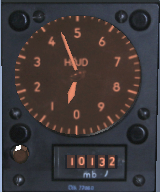
\includegraphics[width=\textwidth]{images/instruments/altimeter}}

\sidepicture{
  \paragraph{Airspeed/Mach Indicator (\figref{fig:front-panel}{item:airspeed})}
  The airspeed indicator is graduated in km/h on a pseudo-logarithmic scale,
  up to \ifbool{AJS}{1400}{1500}km/h.
  The airspeed indicator is fully mechanical.

  The digital Mach indicator has a range of M 0--2.5. It is partially covered at M <0.4.
  The Mach indicator requires AC power.
  A red-white flag indicates power failure of the Mach indicator (but not of the airspeed indicator).

  \AJSonly{
    The knob controls an index on the airspeed scale, with no functionality.
  }
}{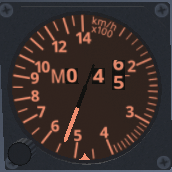
\includegraphics[width=\textwidth]{images/instruments/airspeed}}


\ifbool{AJS}{
\sidepicture{
  \paragraph{Heading Indicator (\figref{fig:front-panel}{item:CI})}
  The heading indicator forms a ring around the radar display (CI).
  The heading scale ring itself rotates, and is read against a fixed index.
  A second yellow moving index indicates bearing to the next waypoint.
  The heading indicator requires AC power. A red-white flag indicates power failure.


}{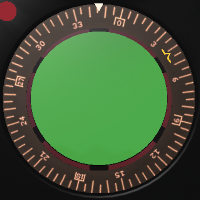
\includegraphics[width=\textwidth]{images/instruments/heading-AJS}}
}{
\sidepicture{
  \paragraph{Heading Indicator (\figref{fig:front-panel}{item:heading})}
  The heading scale itself rotates to indicate aircraft heading, read against a fixed index.
  The thin pointer indicates commanded heading, or bearing to the destination.
  The wide pointer indicates track angle to the target, or runway direction (at landing).
  The heading indicator requires AC power. A red-white flag indicates power failure.

  The heading indicator can also display the output of the backup gyrocompass, cf.~\cref{sec:backup-heading}.
}{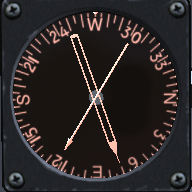
\includegraphics[width=\textwidth]{images/instruments/heading-JA}}
}

\sidepicture{
  \paragraph{Attitude/Director Indicator (\figref{fig:front-panel}{item:adi})}
  The ADI consists of a sphere which rotates in 3 axes, indicating pitch, roll, and course.
  The two flight director needles (horizontal and vertical) show ILS deviation for landing.
  The ADI requires AC power. A red flag indicates power failure.
}{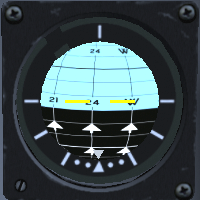
\includegraphics[width=\textwidth]{images/instruments/adi}}

\sidepicture{
  \paragraph{Angle-of-Attack Indicator (\figref{fig:front-panel}{item:aoa})}
  The AoA indicator is graduated in degrees, from -4\textdegree{} to 30\textdegree{}.
  When on the ground, the indicator displays pitch angle instead of AoA.
  The AoA indicator requires DC power.
  In case of power failure, the pointer returns to the -4\textdegree{} position.
}{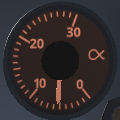
\includegraphics[width=0.8\textwidth]{images/instruments/alpha}}

\sidepicture{
  \paragraph{Accelerometer (\figref{fig:front-panel}{item:gmeter})}
  The accelerometer shows G-load (acceleration along the vertical axis), between -2g and +9g.
  A second pointer shows the maximum (positive) acceleration reached.
  The button resets the maximum acceleration pointer.
  The accelerometer is fully mechanical.
}{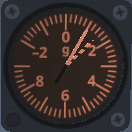
\includegraphics[width=0.7\textwidth]{images/instruments/accelerometer}}


\sidepicture{
  \paragraph{Chronometer \ifbool{AJS}{(\figref{fig:front-panel}{item:clock})}{(\figref{fig:right-panel}{item:clock})}}
  The chronometer has two scales. The inner scale and the white pointers indicate time.
  The outer scale and the yellow pointers are used for the stopwatch.
  The lower-left knob is used to adjust time.
  The top-right button controls the stopwatch.
  The first push starts the stopwatch, the second push stops it, and the third push resets it.
}{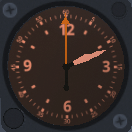
\includegraphics[width=0.7\textwidth]{images/instruments/clock}}

\AJSonly{
\sidepicture{
  \paragraph{Waypoint Distance Indicator (\figref{fig:front-panel}{item:wpdist})}
  Indicates the distance to the next waypoint.
  At distances <40km, the scale is graduated in km.
  At distances >40km, the scale is graduated in Nordic miles (1mil = 10km), and indicates distances up to 400km.
  A small screen indicates the unit in use, as either `km' or `mil'.
}{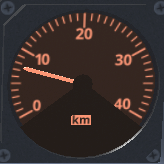
\includegraphics[width=0.8\textwidth]{images/instruments/distance}}

\sidepicture{
  \paragraph{Destination Indicator (\figref{fig:front-panel}{item:wpnum})}
  Indicates the type and number of the next waypoint.
  The first character indicates waypoint type: B for regular waypoints,
  L for departure and landing bases.
  The second character indicates the waypoint number, or S for the departure base.
}{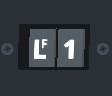
\includegraphics[width=0.7\textwidth]{images/instruments/waypoint}}
}

\section{Backup Instruments}
\sidepicture{
  \paragraph{Backup Altimeter (\figref{fig:front-panel}{item:altimeter-bck})}
  The long pointer is graduated in 100m, the short one in 1000m.
  The indicator can only display altitudes in the range 0--10km, after which it will cycle back to 0.
  The knob is used to set reference pressure, which is displayed in hPa on a digital counter.
  The backup altimeter is fully mechanical.
}{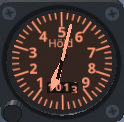
\includegraphics[width=0.7\textwidth]{images/instruments/altimeter_backup}}

\AJSonly{
\sidepicture{
  \paragraph{Backup Airspeed Indicator (\figref{fig:front-panel}{item:airspeed-bck})}
  The backup airspeed indicator is graduated in km/h on a pseudo-logarithmic scale, up to 800km/h.
  It is fully mechanical.
}{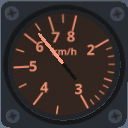
\includegraphics[width=0.7\textwidth]{images/instruments/airspeed_backup}}

\sidepicture{
  \paragraph{Backup Heading Indicator (\figref{fig:front-panel}{item:heading-bck})}
  The backup heading pointer indicates aircraft heading on a fixed scale.
  The backup heading indicator requires AC power.
}{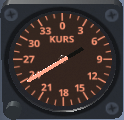
\includegraphics[width=0.7\textwidth]{images/instruments/heading_backup}}
}

\JAonly{
\paragraph{Backup Heading Indicator (\figref{fig:front-panel}{item:heading-bck-but})}
\label{sec:backup-heading}
The JA 37 does not have a separate backup heading indicator.
Instead the main heading indicator can display the output of the backup gyrocompass.
The button BACKUP HEADING (RESERVKURS) toggles this functionality.
When the button light is lit, backup heading is displayed.
The backup gyrocompass requires AC power.
}

\sidepicture{
  \paragraph{Backup Attitude Indicator (\figref{fig:front-panel}{item:attitude-bck})}
  The backup horizon indicates pitch and roll angles.
  The display is mechanical, but the gyro uses AC power.
  A red-white flag indicates power failure.
  The instrument will continue to function with reasonable accuracy for a few minutes after loss of AC power.
}{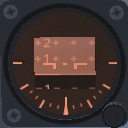
\includegraphics[width=0.7\textwidth]{images/instruments/adi_backup}}

\section{Engine Instruments}
\sidepicture{
  \paragraph{RPM Indicator (\figref{fig:front-panel}{item:rpm})}
  The RPM indicator shows the high pressure compressor speed (N2), on a scale graduated up to 110\%.
  It requires AC power.
}{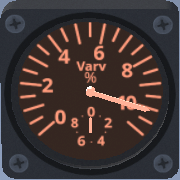
\includegraphics[width=0.7\textwidth]{images/instruments/rpm}}

\sidepicture{
  \paragraph{Engine Pressure Ratio Indicator (\figref{fig:front-panel}{item:epr})}
  The EPR indicator shows the pressure ratio between the intake and the outlet of the turbine
  (before the afterburner stage).
  It requires AC power.
}{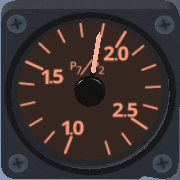
\includegraphics[width=0.7\textwidth]{images/instruments/epr}}

\sidepicture{
  \paragraph{Exhaust Gas Temperature Indicator (\figref{fig:right-panel}{item:egt})}
  The EGT gauge indicates gas temperature after the turbine
  (before the afterburner stage) in \textdegree{}C.
  It requires DC power.
}{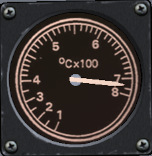
\includegraphics[width=0.7\textwidth]{images/instruments/egt}}

\sidepicture{
  \paragraph{Nozzle Position Indicator (\figref{fig:right-panel}{item:nozzle})}
  The nozzle indicator shows the position of the engine exhaust nozzle and the current afterburner zone.
  It requires DC power.
}{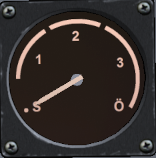
\includegraphics[width=0.7\textwidth]{images/instruments/nozzle}}

\sidepicture{
  \paragraph{Afterburner Zone Indicator (\figref{fig:front-panel}{item:zone})}
  The afterburner zone lights activate to indicate the afterburner zones (1 to 3)
  commanded by the throttle lever position.
  The lights are commanded purely by the throttle position,
  and not the afterburner zones which are actually lit:
  for instance moving the throttle in the afterburner zone during thrust reverse
  causes the lights to activate, despite afterburner being inhibited during reverse.
}{
\includegraphics[width=\textwidth]{images/instruments/zone}}

\sidepicture{
  \paragraph{Fuel Gauge (\figref{fig:front-panel}{item:fuel})}
  The fuel gauge indicates fuel quantity as a percentage.
  Under standard conditions, the gauge indicates \ifbool{AJS}{107}{112}\% with full internal tanks,
  and \ifbool{AJS}{132}{136}\% with the external tank in addition.
  A second black-white pointer indicates required fuel quantity (not implemented).
  The fuel gauge requires AC power.
}{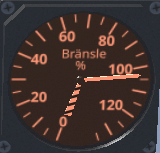
\includegraphics[width=\textwidth]{images/instruments/fuel}}

\section{Warning Lights Panels}
\begin{figure}[ht!]
  \centering
  \includegraphics[width=0.40\textwidth]{
    \ifbool{AJS}{images/panels/AJS-left-warning-panel}{images/panels/JA-left-warning-panel}
  }
  \includegraphics[width=0.40\textwidth]{
    \ifbool{AJS}{images/panels/AJS-right-warning-panel}{images/panels/JA-right-warning-panel}
  }
  \caption{Left and right warning panels (\figref{fig:front-panel}{item:left-warning,item:right-warning})}
  \label{fig:warning-panels}
\end{figure}

\subsection*{Left Side}
\begin{tabular}{llp{0.45\textwidth}}
  Swedish & English & Description \\
  \hline
  BRAND       & FIRE        & Engine fire \\
  BRÄ UPPF    & FUEL DIST   & Fuel distributor failure \\
  X-TANK BRÄ  & X-TANK FUEL & External tank pump low pressure \\
  TANK PUMP   & TANK PUMP   & Fuel feed pump low pressure \\
  LANDSTÄLL   & GEAR        & Steady: landing gear in movement. \\
              &             & Blinking: gear failure, or gear retracted at low speed and altitude. \\
  FÖRV FÖRBJ  & NO REVR ARM & Risk of reverser engaging without WoW \\
  NOS-/V-/H-STÄLL & NOSE-/L-/R-GEAR & Gear down and locked \\
\AJSonly{
  TIPP VÄXEL  & PITCH GEAR  & Elevator reduction gearing failure. \\
}
  \ifbool{AJS}{ELFEL}{ELFÖRS} & ELEC FAIL & Failure of electrical system \\
\ifbool{AJS}{
  RESERVEFF   & RES POWER   & Backup hydraulic pump low pressure or emergency ram air turbine failure \\
}{
  ELREVERS    & ELEC RES    & Emergency ram air turbine failure \\
}
  HYDR-TR 1/2 & HYD PRESS 1/2 & Low pressure in main hydraulic systems \\
  AFK \AJSonly{FEL} & A/T \AJSonly{FAIL} & Steady: auto-throttle disengaged.  \\
              &             & Blinking: A/T failure or abnormal disengagement. \\
  EJ REV      & NO REVR     & Reverser or tertiary air intake failure \\
\JAonly{
  HYDRRESERV  & HYD RES     & Backup hydraulic pump low pressure \\
}
  OLJETRYCK   & OIL PRESS   & Low pressure in engine oil system \\
  OLJETEMP    & OIL TEMP    & High engine oil temperature
\end{tabular}

\subsection*{Right Side}
\begin{tabular}{llp{0.45\textwidth}}
  Swedish & English & Description \\
  \hline
  SPAK        & STICK       & Stability assist failure (press any autopilot button to reset after acknowledgment) \\
\ifbool{AJS}{
  HÅLL-FUNK   & AUTOPILOT   & Autopilot failure (idem) \\
  RHM FEL     & RAD ALT FAIL& Radar altimeter failure \\
  ROLL VÄXEL  & ROLL GEAR   & Roll reduction gearing failure \\
  CK          & COMPUTER    & Primary computer failure \\
}{
  ATT         & ATT         & Attitude hold failure (idem) \\
  HÖJD        & ALT         & Altitude hold failure (idem) \\
  BRAND GTS   & FIRE GTS    & Engine starter turbine fire \\
  TIPP VÄXEL  & PITCH GEAR  & Failure of elevation reduction gearing \\
}
  KABINHÖJD   & CABIN ALT   & Low cabin pressure \\
  HUV o STOL  & CANOPY/SEAT & Canopy open or ejection seat disarmed \\
  TÄNDSYS     & IGN SYS     & Engine ignition system active \\
  STARTSYST   & START SYS   & Starting sequence in progress \\
  MAN BR REG  & MAN FUEL    & Manuel fuel injection regulation \\
\JAonly{
  CD          & COMPUTER    & Primary computer failure \\
  PRIMÄRDATA  & PRI DATA    & Flight data computer failure \\
  TN          & INS         & Inertial navigation central failure \\
  RADAR       & RADAR       & Radar failure \\
  IKS         & IFF         & Military identification transponder failure \\
  ALFA        & ALPHA       & Angle-of-attack sensor failure \\
}
  SYRGAS      & OXYGEN      & Oxygen mask low pressure \\
\ifbool{AJS}{
  BRÄ < 24    & FUEL < 24   & Low fuel quantity \\
  BRAND GTS   & FIRE GTS    & Engine starter turbine fire \\
  TILS        & TILS        & Receiving TILS signal (blinking: no vertical signal) \\
  NAV-SYST    & NAV-SYS     & Navigation systems failure \\
  KB-V SLUT   & KB-L QTY    & Low chaff quantity in left pod (blinking at 10\%, steady when empty) \\
  KB-H/KA SL  & KB-R/KA QTY & Low chaff quantity in right pod (idem), or failure of KA / U-22 ECM pod \\
  FACKL SL    & FLARES QTY  & Low flares quantity (idem) \\
  MOTVERK     & CHAFF/ECM   & Releasing chaffs or ECM pod active \\
  LUFTBROMS   & AIR BRAKES  & Air brakes extended \\
}{
  UTL TEMP    & EXH TEMP    & High exhaust gas temperature \\
  BRÄ MÄNGD   & FUEL QTY    & Low fuel quantity \\
  ANP 37      & ANP 37      & Weapon computer failure
}
\end{tabular}

\section{Other Indicator Lights}
\paragraph{Master Warning (\figref{fig:front-panel}{item:master-warning})}
The master warning consists of two flashing red lights,
\ifbool{AJS}{together with a sound warning.}{sometimes accompanied by a sound warning, depending on the cause.}
It generally lights up together with a blinking light on the warning panels.
Pressing the button between the lights acknowledges the warning,
which causes the corresponding light on the warning panels to become steady.

\paragraph{Reverser (\figref{fig:front-panel}{item:rev-light})}
Green light, indicates that the reverser handle
(\figref{fig:front-panel}{item:rev-handle}) is pulled,
and the reverser is armed (but not necessarily active).

\paragraph{Autopilot (\figref{fig:front-panel}{item:autopilot})}
Three green pushbuttons/lights.
Used to select one of the autopilot modes: stability assist (STICK/SPAK),
attitude hold (ATT), altitude hold (ALT/HÖJD).
When an autopilot mode is active, the light for it and any lower mode are lit.
The lights can blink to indicate special flight conditions under which the
autopilot is not fully functional.

\paragraph{Autothrottle (\figref{fig:front-panel}{item:autothrottle-lights})}
The orange A/T (AFK) light indicates that autothrottle is active.
The pushbutton/light 15,5\textdegree{} is used to select the high-alpha landing mode
(requires landing gear down).

\paragraph{Transonic / Low Speed Reverse(\figref{fig:front-panel}{item:transonic})}
Yellow light, indicates that the aircraft is in the transonic regime.

On the ground, it instead indicates that the reverser is active at low airspeed,
causing a risk of hot air ingestion and engine fire.
A low throttle setting (EPR<1.4) should be maintained in this case.

\AJSonly{
\paragraph{Weapon Released (\figref{fig:front-panel}{item:release})}
When using Rb 04, Rb 15, and m/71, a steady light indicates that the weapon release sequence is complete.
The light goes off when securing the trigger safety.

A blinking light indicates that a weapon was not properly released.
}

% Not implemented
%\paragraph{Fast Reset (\figref{fig:front-panel}{item:fast-reset})}}


\chapter{Control Panels}

\AJSonly{
\sidepicture{
  \section{Main Mode Selector}
  The main mode selector knob \figref{fig:left-panel}{item:main-mode}
  is located on the radar panel, next to the throttle.
  It selects an aircraft main operation mode, corresponding to different phases of a flight.
  The knob can be rotated with the keybindings \keys{M} / \keys{\shift+M}.
}{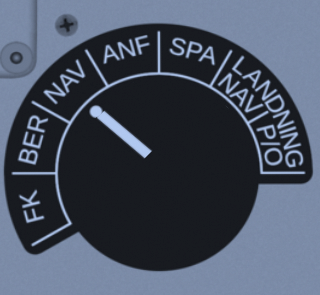
\includegraphics[width=\textwidth]{images/controls/mode-selector}}

\begin{description}
  \item[FK/TST] Built-in test. Not implemented (does the same as BER/PRE).
  \item[BER/PRE] Standby mode used for start-up and taxi.  Displays (HUD and CI) are turned off.
  \item[NAV] Navigation mode. Used during most of the flight, including takeoff.
  \item[ANF/CBT] Combat mode. See \cref{chap:weapons}.
  \item[SPA/REC] Reconnaissance mode. Not implemented (does the same as NAV).
  \item[LANDING NAV] Instruments landing mode.
    Enables landing guidance using inertial navigation and ILS,
    provided the destination is set in the route manager.
  \item[LANDING P/O] Visual landing mode.
\end{description}

A typical flight may use the following modes.
Initially, the mode is BER/PRE.
Shortly before takeoff (when entering the runway), the mode is switched to NAV.
In order to use weapons, the mode is switched to ANF/CBT,
then back to NAV when resuming normal flight.

LANDING mode is typically selected within 20km of the destination.
LANDING NAV mode will give indications to follow a full approach pattern,
and enables ILS guidance for final, if available.
LANDING P/O simply gives indicates runway heading and nominal glide slope on the HUD, for visual landing.
One can also begin the approach in LANDING NAV mode,
and later switch to LANDING P/O to finish the approach visually.

For the LANDING NAV mode, the approach pattern can be changed
by the following operations (called `flip-flop').
\begin{itemize}
  \item Switching to LANDING P/O, then back to LANDING NAV select the short approach mode,
    with a 10km final instead of a 20km final.
  \item Switching to NAV, then back to LANDING NAV
    starts a new approach pattern, with a long (20km) final.
    (NAV can be replaced by any non-landing mode).
\end{itemize}
}

\section{Radios}
\ifbool{AJS}{
  The \variant{} is equipped with two communication radios:
  the FR 22 primary radio, and the FR 24 backup radio.

  The FR 22 operates in the VHF band 103.000--155.975 MHz with 25KHz spacing,
  and in the UHF band 225.000--399.950 MHz with 50KHz spacing.
  It can use 762 programmable channels, as well as direct frequency input.

  The FR 24 operates in the VHF band 110.000--147.000 MHz with 50KHz,
  and is restricted to 4 pre-programmed channels.
  The FR 24 can be powered by the aircraft battery.
}{
  The \variant{} is equipped with two communication radios.

  The FR 29 primary radio operates in the VHF band 103.000--159.975 MHz
  and in the UHF band 225.000--399.975 MHz, both with 25KHz spacing.
  It consists of two FR 28 transceivers, called A and B.
  At all time, one transceiver is used for voice communication, while the other is used for data link.
  Transceiver B (unlike A) can be powered by the aircraft battery,
  and should thus be used when AC power is unavailable,
  on the ground before startup or in case of electrical failure.
  The FR 29 can use 934 programmable channels, as well as direct frequency input.

  The FR 31 secondary radio operates in the VHF band 104.000--161.975 MHz
  and in the UHF band 223.000--407.975 MHz, both with 25KHz spacing.
  It can use 971 programmable channels, as well as direct frequency input.
}

\subsection{FR \ifbool{AJS}{24}{29} Radio Panel}
\ifbool{AJS}{%
  The FR 24 radio panel (\figref{fig:left-panel}{item:fr29}) is used to set
  the operating mode and volume of both the FR 22 and FR 24, as well as the FR 24 channel.
  In FlightGear, it is not correctly modelled, and is replaced by the FR 29 panel
  from the JA variant, which has a similar purpose.
}{
  The FR 29 radio panel (\figref{fig:left-panel}{item:fr29}) is used to set 
  the operating mode and volume of the FR 29.
}
\begin{figure}[h]
  \centering
  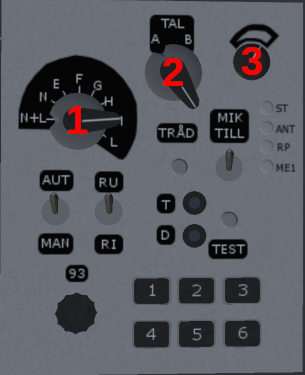
\includegraphics[width=0.4\textwidth]{images/controls/fr29.png}

  \begin{enumerate}[nosep]
    \item \label{item:knob-mode} Mode / channel knob
    \item \label{item:knob-transceiver} \ifbool{AJS}{No functionality on AJS}{Select FR 28 transceiver A/B}
    \item \label{item:knob-volume} Volume knob. Inner knob sets \ifbool{AJS}{FR 22 and FR 24}{FR 29} volume.
      Outer knob sets warnings volume.
  \end{enumerate}
  \caption{FR \ifbool{AJS}{24}{29} Radio Panel}
  \label{fig:fr29}
\end{figure}

The radio operation modes, selected with the \ifbool{AJS}{FR 24}{FR 29} panel knob
(\figref{fig:fr29}{item:knob-mode}) are the following.
\begin{description}
  \item[N+L (NORM+LARM)] \ifbool{AJS}{%
      FR 22 radio is active, its frequency is set with the FR 22 channel and frequency selectors.
      FR 24 acts as a receiver for the guard channel 121.5MHz.
    }{%
      Frequency is set with the KV1 channel selector.
      An additional receiver integrated in the FR 28 monitors the guard channel 121.5MHz.
    }
  \item[N (NORM)] Same as N+L, without the guard channel receiver\AJSonly{. FR 24 is inactive}.
  \item[E,F,G,H] Sets the corresponding global channel\AJSonly{ for the FR 24.  FR 22 is inactive}.
  \item[M,L] \ifbool{AJS}{No functionality.}{Sets the corresponding custom channel.}
\end{description}

\ifbool{AJS}{
  \subsection{FR 22 Channel and Frequency Selectors}
  Frequency or channel for the FR 22 radio is set through the
  FR 22 channel selector (\figref{fig:left-panel}{item:fr22})
  and frequency selector (\figref{fig:front-panel}{item:frequency-sel}).

  \begin{figure}[h]
    \centering
    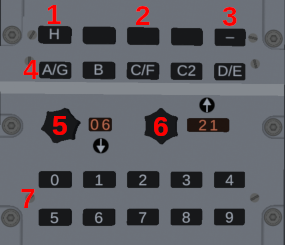
\includegraphics[width=0.5\textwidth]{images/controls/fr22.png}

    \begin{enumerate}[nosep]
      \item \label{item:channel-guard} Guard channel H.
      \item \label{item:channel-special} Special channels S1,S2,S3 (unlabelled buttons).
      \item \label{item:channel-freq} Frequency selector button `--'.
      \item \label{item:channel-base} Airbase channel buttons A/G, B, C/F, C2, D/E.
      \item \label{item:knob-group} Channel group knob and display (showing channel group 06).
      \item \label{item:knob-base} Airbase knob and display (showing airbase 21).
        Every sixth position shows ALLM/GEN.
      \item \label{item:channel-group} Channel buttons 0 to 9.
    \end{enumerate}
    \caption{FR 22 channel selector panel}
    \label{fig:fr22}
  \end{figure}

  To directly select a frequency, press button `--' (\figref{fig:fr22}{item:channel-freq})
  and set the frequency on the frequency selector panel.
  Note that invalid frequencies can be set (e.g.\ outside of the FR 22 bands,
  or with invalid spacing in the UHF band) in which case the FR 22 will not work.

  To select the guard channel H (121.5MHz) or one of the special channels S1,S2,S3,
  press the corresponding button (\figref{fig:fr22}{item:channel-guard} or
  \figref{fig:fr22}{item:channel-special}).

  To select an airbase channel, set the airbase number with the airbase knob (\figref{fig:fr22}{item:knob-base})
  and select the channel with one of the airbase channel buttons (\figref{fig:fr22}{item:channel-base}).
  For instance, set the airbase number to 21 and press button A/G for channel 21A.

  To select one of the global channels E,F,G, set the airbase knob (\figref{fig:fr22}{item:knob-base})
  to one of the positions ALLM (every 6th position), and select the channel
  with one of buttons A/G, C/F, D/E (\figref{fig:fr22}{item:channel-base}).

  To select a generic channel, set the channel group with the group knob (\figref{fig:fr22}{item:knob-group})
  and select the channel with one of the channel buttons (\figref{fig:fr22}{item:channel-group}).
  For instance, set the group number to 06 and press button 2 for channel 062.
}{
  \subsection{KV1 and KV3 Channel Selectors}
  The KV1 (\figref{fig:left-panel}{item:kv1}) is used to set the channel of frequency for the FR 29 comm radio.
  The KV3 (\figref{fig:left-panel}{item:kv3}) is used to set the datalink channel.

  \begin{figure}[h]
    \centering
    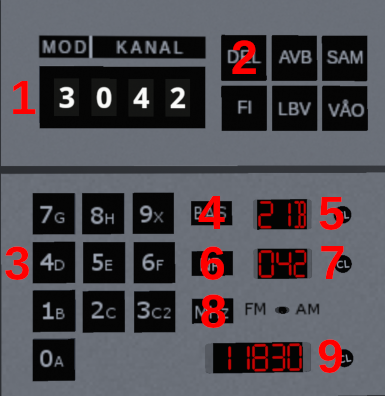
\includegraphics[width=0.5\textwidth]{images/controls/kv1.png}

    \begin{enumerate}[nosep]
      \item \label{item:kv3-display} KV3 datalink identifier and channel display.
      \item \label{item:kv3-clear} KV3 `clear display' button.
      \item \label{item:kv1-keypad} Input keypad.
      \item \label{item:kv1-base-button} Airbase channel mode button.
      \item \label{item:kv1-base-screen} Airbase channel input screen and clear button.
      \item \label{item:kv1-nr-button} Generic channel mode button.
      \item \label{item:kv1-nr-screen} Generic channel input screen and clear button.
      \item \label{item:kv1-mhz-button} Frequency mode button.
      \item \label{item:kv1-mhz-screen} Frequency input screen and clear button.
    \end{enumerate}
    \caption{KV1 and KV3 channel selector panels}
    \label{fig:kv1}
  \end{figure}

  To enter a frequency or channel on one of the four screens
  (\figref{fig:kv1}{item:kv3-display,item:kv1-base-screen,item:kv1-nr-screen,item:kv1-mhz-screen}),
  press the corresponding `clear' button and input the new value using the KV1 keypad
  (\figref{fig:kv1}{item:kv1-keypad}).
  \begin{itemize}[noitemsep]
    \item Airbase channels are input in the format XXC, where XX is the airbase number, and C is the channel letter.
      For instance channel 21B is selected in \cref{fig:kv1}.
      If the letter is E,F, or G, the airbase number is ignored and the
      corresponding global channel is selected, e.g.\ 21E will select channel E.
    \item Generic channels are input with three digits. Channels 000--429 can be used.
    \item Frequencies are input with five digits, rounded down to 10KHz,
      For instance frequency 118.300MHz is selected in \cref{fig:kv1}.
      Since frequencies have 25KHz spacing, the last digit must be one of 0,2,5,7.
  \end{itemize}

  The three mode buttons (\figref{fig:kv1}{item:kv1-base-button,item:kv1-nr-button,item:kv1-mhz-button}),
  are used to select whether the airbase channel, generic channel, or frequency is used.
  When a screen is cleared for input, its previous value remains in use until the new input is complete and correct.
  The old value is restored on the screen when pressing the corresponding mode button,
  or if a different screen is cleared for input.
  An erroneous input is indicated by `$\equiv$', and the screen must be cleared to correct it.
  A screen waiting for input will start blinking with symbol `-' after 9 seconds.

  If the airbase or generic channel mode is selected and no screen is waiting for input,
  pressing a keypad button will change the last character of the current airbase,
  respectively generic channel.
  E.g.\ if airbase channel 21A is in use, pressing button 1/B will switch to channel 21B.

  \subsection{FR 31 Radio Panel (\figref{fig:right-panel}{item:fr31})}
  \begin{figure}[h]
    \centering
    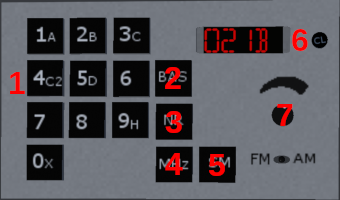
\includegraphics[width=0.6\textwidth]{images/controls/fr31.png}

    \begin{enumerate}[nosep]
      \item \label{item:keypad} Input keypad.
      \item \label{item:base} Airbase channel mode button.
      \item \label{item:nr} Generic channel mode button.
      \item \label{item:mhz} Frequency mode button.
      \item \label{item:backup-ptt} Backup PTT button (not implemented).
      \item \label{item:screen} Input screen and clear button.
      \item \label{item:vol} Volume knob.
    \end{enumerate}
    \caption{FR 31 radio panel}
    \label{fig:fr31}
  \end{figure}
  To enter a frequency or channel, select the airbase channel, generic
  channel, or frequency mode with the respective buttons if it is different
  from the current mode, (\figref{fig:fr31}{item:base,item:nr,item:mhz}),
  then press the `clear' button and enter the new value with the keypad (\figref{fig:fr31}{item:keypad}).
  The previous channel or frequency remains in use until the new input is complete.
  Invalid key presses are ignored.
  \begin{itemize}[noitemsep]
    \item Guard channel H is selected by entering a single H, in any mode.
    \item Airbase channels are input in the format XXXC,
      where XXX is the airbase number, and C is the channel letter.
      Airbase numbers 000--169 can be used.
    \item Generic channels are input with three digits. Channels 000--119 can be used.
    \item Frequencies are input with five digits, rounded down to 10KHz.
      Since frequencies have 25KHz spacing, the last digit must be one of 0,2,5,7.
  \end{itemize}
}

\subsection{Radio Channels}
The different Viggen radios can use a number of configurable radio channels.
Available channel names are the following.
\begin{description}
  \item[Generic channels] These channels are normally used to communicate between aircrafts, and with fighter control.
    Their name consists of 3 digits.
    \ifbool{AJS}{%
      Channels 010 to 419 can be used.
    }{%
      The FR 29 can use channels 000 to 429, and the FR 31 can use channels 000 to 119.
    }
  \item[Airbase channels] These channels are normally used to communicate with ATC.
    Their name consists of an airbase number (2 digits),
    followed by one of the letters A,B,C,C2,D.
    \ifbool{AJS}{%
      Airbase numbers 01 to 69 can be used.
    }{%
      The FR 29 can use airbase numbers 00 to 99, and the FR 31 can use airbase numbers 000 to 169
      (airbase numbers have an additional leading digit on the FR 31).
    }
  \item[Guard channel] The international guard channel 121.5MHz, called channel H.
  \item[Global channels] Three fixed, global channels, called E,F,G\JAonly{ (unavailable on the FR 31)}.
  \item[Others] \ifbool{AJS}{%
      The FR 22 has three unlabelled channel buttons, nicknamed S1,S2,S3 in this manual.
    }{%
      The FR 29 has two programmable channels called M,L.
    }
\end{description}

These channels (except for guard channel H) are defined in text configuration files,
which can be loaded through \menu{\variant{}>Load radio channels}.
Configuration file syntax is described in \directory{Aircraft/JA37/Doc/channels-example.txt}.
By default the file \directory{Aircraft/JA37/Nasal/radios/channels-default.txt} is loaded.


\JAonly{
  \subsection{Data Link}
  Data link is used to communicate data such as position of friendly aircrafts
  and of targets with ground control (STRIL) and between fighters (fighter link).
  A very limited part of fighter link is implemented, allowing aircrafts to share their position,
  and the position of aircrafts they are tracking.
  This information is displayed on the TI.

  Datalink is activated with the DL button in the SYST page on the TI.
  The KV3 screen (\figref{fig:kv1}{item:kv3-display}) is used to set the datalink channel
  on the last 3 digits, and a datalink identifier on the first digit.
  Aircrafts must be on the same datalink channel to communicate.
  The identifier helps to distinguish between aircrafts on a same datalink channel.
  Each aircraft should set it to a different number, (e.g.\ its position in the formation).
  The identifier is ignored if it is 0.

  \newcommand{\dlfriend}{%
    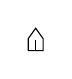
\begin{tikzpicture}%
      \draw (0,0) -- (0,1ex) -- (0.625ex,1.875ex) -- (1.25ex,1ex) -- (1.25ex,0) -- (0,0);
      \draw (0.625ex,0) -- (0.625ex,0.875ex);
    \end{tikzpicture}%
  }
  \newcommand{\dltarget}{%
    
\begin{tikzpicture}%
      \draw (0,1ex) circle (1ex);
      \draw (0,0.5ex) circle (0.5ex);
    \end{tikzpicture}%
  }

  On the TI, an aircraft connected through datalink shows
  as a green \dlfriend{} with its identifier below it, if any.
  Furthermore, an aircraft A connected through datalink
  may transmit information about an aircraft B which it is tracking.
  Then, aircraft B is displayed as \dltarget{} with the identifier of A below it, if any.
}


\section{Identification Friend or Foe (IFF)}
\label{sec:iff}
IFF is a radar system designed to identify friendly aircrafts.%
\footnote{%
  Despite the name, IFF can by no mean identify foes.
  An enemy aircraft is undistinguishable from e.g.\ a civilian aircraft,
  or an aircraft with a non-functioning IFF system.
}
Each aircraft can set a \emph{query code} for its IFF system,
and aircrafts with the same query code set will be identified as friendly.
Thus, allied aircrafts can identify each other by using a shared code, chosen before the mission.
In FlightGear, other aircrafts with a compatible IFF system include the F-16
and Justin Nicholson's MiG-21\footnote{\url{https://github.com/l0k1/MiG-21bis}}.

\AJSonly{
The AJS variant of the Viggen is only equipped with the transponder part of the IFF system:
it can be identified by other aircrafts, but can not identify them.
}

\noindent
\begin{minipage}[t]{0.55\textwidth}
  \vspace{0pt}
  \setlength{\parindent}{1em}
  \paragraph{Control Panel}
  The IFF control panel \figref{fig:right-panel}{item:iff}
  is located on the rear right side of the cockpit.
  The right knob is the power knob, with 3 positions: OFF/FRÅN, AUTO (on when airborne), ON/TILL.
  The left knob is used to set the query code, between 1 and 11.
\end{minipage}
\hspace{0.1\textwidth}
\begin{minipage}[t]{0.35\textwidth}
  \vspace{0pt}
  \centering
  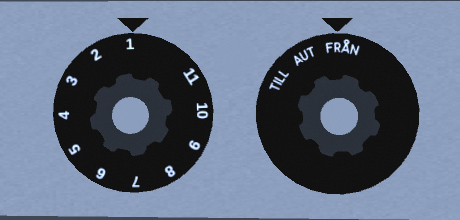
\includegraphics[width=\textwidth]{images/controls/iff.png}
\end{minipage}

\JAonly{
\paragraph{Identification of Contacts}
IFF interrogation is done with \keys{N}, and lasts 10 seconds, during which the IK light on the MI frame is lit.
The IFF radar is a secondary radar physically tied to the primary radar,
which will interrogate any contact in the primary radar search area.
Friendly responses are displayed with a cross on the MI.

For any tracked radar contact, the IFF response or lack thereof is stored, as long as tracking is maintained.
It is displayed on the HUD and the TI with a cross over friendly contacts.
Additionally, the TI uses a color code: green for friendly contacts,
red for contacts which failed to answer an IFF interrogation,
and yellow for contacts which were not interrogated.
The IFF information displayed on the TI and HUD can also use information transmitted by other aircrafts on datalink.

\paragraph{Friendly Callsigns}
The menu \menu{JA-37Di>Friends (IFF)} allows to set a list of friendly callsigns.
Aircrafts with these callsigns will always be identified as friendly by IFF,
even if they do not have the same IFF query code.
This allows to operate with other aircrafts which do not have a compatible IFF system.
}

\AJSonly{
\section{Weapon Panel}
\label{sec:weapon-panel}
The weapon panel (\figref{fig:right-panel}{item:wpn-panel})
is used to select weapons and adjust their settings.

\begin{figure}[ht]
  \centering
  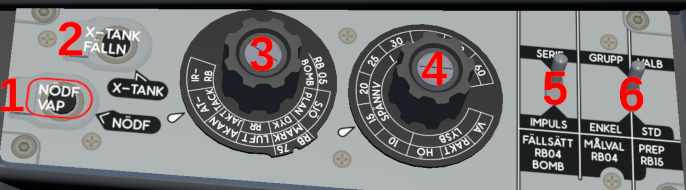
\includegraphics[width=0.9\textwidth]{images/controls/AJS-weapon-panel.png}

  \begin{multicols}{2}
    \begin{enumerate}[nosep]
      \item \label{item:jett-payload} Jettison payload button (guarded)
      \item \label{item:jett-tank} Jettison fuel tank (guarded)
      \item \label{item:wpn-sel} Weapon selection knob
      \item \label{item:dist-sel} Wingspan / bomb interval selection knob
      \item \label{item:impuls} Sequence release / ARAK long range
      \item Missile search pattern settings (not implemented)
    \end{enumerate}
  \end{multicols}
  \caption{Weapons panel}
  \label{fig:wpn-panel}
\end{figure}

\paragraph{Jettison Buttons}
There are two jettison buttons, guarded by a cover.
The first (\figref{fig:wpn-panel}{item:jett-payload}) jettisons all external load,
except for the outer wing pylons.
The second (\figref{fig:wpn-panel}{item:jett-tank}) jettisons only the external fuel tank.

\paragraph{Weapon Selector}
The weapon selection knob (\figref{fig:wpn-panel}{item:wpn-sel}) is used to select weapon types,
as well as special aiming modes for some weapons.
The positions allow to select the following weapons.
\begin{description}
  \item[IR-RB] Rb 24, Rb 24J, and Rb 74 Sidewinders
  \item[ATTACK] AKAN cannon pods, ARAK rocket pods, Rb 04, Rb 15, or m/90
  \item[AKAN JAKT] AKAN cannon pods with A/A aiming mode
  \item[LUFT / RR] Rb 05 with A/A aiming mode, or bombs with radar aiming mode.
  \item[RB 75 / MARK / DYK] Rb 75, or Rb 05 in A/G mode, or bombs with dive aiming mode.
  \item[SJÖ / PLAN] Rb 05 in A/S mode, or bombs with level release aiming mode.
\end{description}

Remarks:
\begin{itemize}
  \item Most positions can be used to select several weapons.
    This means that these weapons are mutually exclusive (they can not be loaded together).
    See \cref{sec:loadout} for more details.
  \item Position IR-RB is an exception: different types of sidewinders can be loaded together,
    and are selected simultaneously by this position.
    Use button IR-RB FRAMSTEGN (\figref{fig:left-panel}{item:ir-framstegn}) to cycle pylons.
  \item The different bomb aiming modes are not implemented. Only a generic CCIP exists.
  \item Rb 05 MARK and SJÖ modes differ only by the fuse setting, which is not implemented.
\end{itemize}

\paragraph{Wingspan and Bomb Interval Selector}
This knob (\figref{fig:wpn-panel}{item:dist-sel}) is used to set the bomb release interval,
and the target wingspan for the HUD in A/A aiming modes. It is graduated in meters from 10m to 60m.
The three leftmost positions (VÄ, RAKT, HÖ) are used for illumination bombs, which are not implemented.

\paragraph{Sequence Release and ARAK Long Range Mode}
The switch SERIE/IMPULS (\figref{fig:wpn-panel}{item:impuls})
has different functions depending on the selected weapon.
\begin{description}
  \item[Rb 04 / Rb 15] The switch controls sequence release.
    In position SERIE, both missiles are launched with 2 second interval.
    In position IMPULS, only one missile is launched at a time.
  \item[ARAK] The switch controls long range aiming mode.
    In position SERIE, the normal aiming mode is used.
    In position IMPULS, a long range standoff aiming mode is used.
    It allows firing at up to 7km from the target, but with reduced accuracy and more restrictive aiming conditions.
\end{description}
Despite the label, this switch has no functionality for bombs
(it is only used for training bombs, which are not implemented).
}



\chapter{Displays}
\ifbool{AJS}{\section{Generalities}
All primary displays use electrical power from the secondary AC bus.
The displays are turned on when switching the main mode selector
(\cockpitref{fig:left-panel}{item:main-mode}) from BER/PRE to NAV.

Displays require some preheating before being functional:
\begin{itemize}
  \item The HUD can turn on 30 seconds after AC power is available.
  \item The CI can turn on 30 seconds after switching to mode NAV.
\end{itemize}

\section{Head Up Display (HUD)}
\subsection{Overview}
\begin{figure}[!ht]
  \centering
  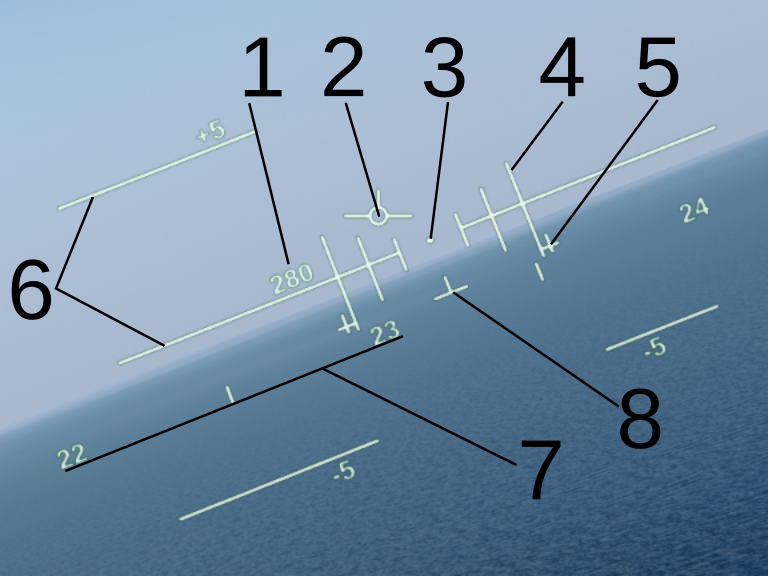
\includegraphics[width=0.6\textwidth]{images/displays/ajs-hud-general.png}

  \begin{multicols}{2}
    \begin{enumerate}[nosep]
      \item \label{item:digalt} Digital altitude
      \item \label{item:fpv} Flight path vector
      \item \label{item:refpt} Reference point
      \item \label{item:alt} Altitude bars
      \item \label{item:refbars} Reference bars and radar altitude index
      \item \label{item:horizon} Artificial horizon and pitch lines
      \item \label{item:heading} Heading scale
      \item \label{item:timeline} Time / distance scale
    \end{enumerate}
  \end{multicols}

  \caption{HUD overview}
  \label{fig:hud}
\end{figure}

\subsection{Controls}
HUD brightness is adjusted with knob \cockpitref{fig:front-panel}{item:hud-bright}.

The following two switches located on the lower right of the HUD
(\cockpitref{fig:front-panel}{item:hud-switch}) affect the HUD presentation.

\paragraph{SLAV SI (SLV HUD)}
In navigation mode, this switch enables a decluttered low-altitude mode when
in position T (ON), see \cref{sec:hud-declutter}.

During optical landing, when in position T (ON), the HUD reference point will
be aligned with the flight path vector, instead of indicating runway heading.

\paragraph{HÖJD CI SI (ALT DISP)}
When in position RHM (RAD), the radar altimeter is used to compute a ground
corrected altitude, which is displayed on the HUD.
Otherwise, displayed altitude is the same as on the main altimeter.

The switch automatically goes back to position LD (BAR) at altitude >2450m
and during landing final phase.

\subsection{Navigation Mode}
\paragraph{Artificial Horizon (\cockpitref{fig:hud}{item:horizon})}
The artificial horizon and the $\pm 5 \degree$ pitch lines provide an attitude reference.
The HUD does not have a full pitch scale, only the horizon and the $\pm 5 \degree$ lines.

Horizontally, the artificial horizon is pointing towards the current destination,
indicated by the reference point (\cockpitref{fig:hud}{item:refpt}).

\paragraph{Flight Path Vector (\cockpitref{fig:hud}{item:fpv})}
The FPV marker indicates the aircraft path direction relative to the ground.
When on the horizon, the aircraft is in level flight.
When covering the reference point, the aircraft track coincides with the destination.

\paragraph{Digital Altitude (\cockpitref{fig:hud}{item:digalt})}
Displays the aircraft altitude.
Below 1km the altitude is displayed in meters with a precision of 10m.
Above 1km the altitude is displayed in kilometers with a precision of 100m.
Above 10km, the digital altitude cycles back to 0,
thus 1500m and 11500m are both displayed as `1,5'.
Negative altitude down to -90m can be displayed.

\paragraph{Altitude Bars (\cockpitref{fig:hud}{item:alt})}
The 6 altitude bars indicate the aircraft altitude relative to the reference altitude
(also called commanded altitude).

The top of the bars represents the reference altitude,
and the bottom of the bars represent ground level (to be exact, indicated altitude 0m).
The aircraft altitude is indicated by the horizon line.
Thus, if the top of the bars is aligned with the horizon, the aircraft is at the commanded altitude,
and if the bottom of the bars is aligned with the horizon, the aircraft is at ground level.

One can imagine the top, resp.\ bottom of the bars as forming a horizontal
plane in a perspective drawing, located at reference altitude, resp.\ ground altitude.
In this perspective drawing, the vanishing point is the reference point.

If the reference altitude is higher than 500m,
the bottom of the bars represents the reference altitude minus 500m instead of ground level.

\subparagraph{Reference Altitude}
The reference altitude displayed by the altitude bars is set as follows.
\begin{itemize}[noitemsep]
  \item During takeoff, reference altitude is fixed at 500m.
  \item During flight, the reference button (keybinding \keys{\shift+R}) 
    sets it to the current altitude.
  \item If autopilot altitude hold mode is active,
    the reference altitude is the autopilot altitude.
  \item When entering landing mode, reference altitude is set to 500m.
    It can still be modified with the reference button or by engaging autopilot altitude hold.
\end{itemize}

If the difference between reference altitude and current altitude is too large,
the displayed reference altitude will differ from the actual reference altitude.

\subparagraph{Reference Altitude Bars (\cockpitref{fig:hud}{item:refbars})}
The reference altitude bars are located just next to the outer altitude bars.
The length of the reference altitude bars varies to indicate reference altitude:
if the length of the outer altitude bars (which is fixed to 3\textdegree{})
represents the reference altitude, then the length of the reference altitude bars represents 100m.

For instance, in \cref{fig:hud}, the length of the reference altitude bars is
0.6\textdegree{}, i.e.\ 1/5 of the outer altitude bars.
Thus 100m is 1/5 of the reference altitude, i.e.\ the reference altitude is 500m.

At reference altitudes higher than 500m, the reference bars are hidden.

\subparagraph{Radar Altitude Index (\cockpitref{fig:hud}{item:refbars})}
When available, radar altitude is indicated by a horizontal index on the outer altitude bars,
which can be read on the outer altitude bars or the reference altitude bars.

When the index is at the bottom of the altitude bars,
radar altitude and indicated altitude coincide,
which can be used to calibrate the altimeter in flight.
However this method is only accurate when reference altitude is at most 500m
(reference altitude bars are displayed).

\paragraph{Heading Scale (\cockpitref{fig:hud}{item:heading})}
Indicates current heading.
Every 10\textdegree{} is indicated by a number,
and every 5\textdegree{} between them by a vertical mark.
The scale is 1:1, i.e.\ the bearing of a world object can be read directly on the scale.

\paragraph{Time and Distance Scale (\cockpitref{fig:hud}{item:timeline})}
Indicate time or distance to an event or waypoint.
The line shrinks and grows horizontally around the center to indicate time or distance to the event.
A vertical center mark, and in some modes two side marks, represent the events.
\begin{itemize}
  \item During takeoff roll, the line grows to indicate aircraft speed.
    The side marks indicate recommended rotation speed.
  \item In navigation mode, the line represents time to the next waypoint.
    It appears 60 seconds before the waypoint, and shrinks until reaching the waypoint.
  \item In cannon or rocket aiming modes, the line indicates distance to target,
    and the side marks indicate minimum firing distance.
\end{itemize}

\subsection{Low Altitude Declutter}
\label{sec:hud-declutter}
If the switch SLAV SI is in position T (TILL), a decluttered HUD is displayed at altitude <100m.
In this decluttered mode, only the flight path vector,
artificial horizon, and digital altitude are displayed.
Pressing the reference button (keybinding \keys{\shift+R})
in decluttered mode toggles the heading scale.

\subsection{Takeoff Mod}
Takeoff mode is enabled is enabled when the nose gear is compressed,
provided the master mode selector is not in mode LANDING.

During takeoff, the FPV is fixed 10\textdegree{} below the aircraft forward axis,
and the FPV marker vertical fin is hidden.
The artificial horizon reference point is aligned with the aircraft forward axis.
Time line and heading scale are fixed 10\textdegree{} below the horizon.
The time line indicates airspeed, with the side markers corresponding to rotation speed.

When the rotation angle reaches 5\textdegree{},
the time line is hidden and the heading scale moves to its normal position.

Takeoff mode stops when the airspeed exceeds M 0.35,
or when the flight path angle is at least 3\textdegree{} up,
or at landing gear retraction.

\subsection{Landing Mode}
\begin{figure}[!ht]
  \centering
  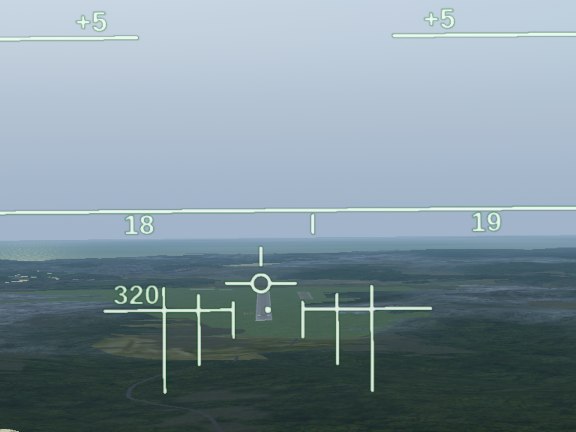
\includegraphics[width=0.5\textwidth]{images/displays/ajs-hud-landing.png}
  \caption{HUD during final}
  \label{fig:hud-landing}
\end{figure}

In landing mode, the HUD changes when starting the final.
The -5\textdegree{} pitch lines are removed,
and a glideslope line is added 2.86\textdegree{} below the horizon
(corresponding to a slope of 5\%).
Altitude bars and digital altitude are moved from the horizon to the glideslope line,
and the heading scale is moved under the horizon.

\paragraph{Speed / AoA Indicator}
In landing mode, the vertical fin (`tail') of the flight path vector symbol
moves vertically to indicate deviation from the target speed or angle of attack.

The speed is correct when the bottom of the tail is on the FPV circle
(default position in navigation mode).
If the tail is higher than the circle, the aircraft speed is too high.
If the tail is lower (inside the circle), the aircraft speed is too low.

While the landing gear is up, the target speed is 550km/h.
Once the landing gear is down and locked, the target angle of attack is 12\textdegree{}.
If the $\alpha 15,5\degree$ button
(\cockpitref{fig:front-panel}{item:autothrottle-lights}) is pressed (light lit),
the target angle of attack is 15.5\textdegree{} instead.

When the landing gear is down, the fin will blink if the angle of attack is critically high.

\paragraph{ILS Guidance}
If ILS guidance is used, the reference point indicates the heading to follow to align with the localizer,
and the altitude bars indicate ILS glideslope deviation:
if the top of the bars is above, resp.\ below the glideslope line,
the aircraft is below, resp.\ above the ILS glideslope.

If ILS is not used (optical landing mode),
the reference point indicates runway heading and the altitude bars are hidden.

\paragraph{Touchdown}
Below 30m, the HUD switches to optical landing display (ILS indications disappear).
Below 15m radar altitude, the HUD switches to flare mode.
The glideslope line moves up to indicate the descent angle
which gives a vertical speed of 2.96m/s, the maximum for touchdown.
If radar altitude is unavailable, transition to flare mode occurs at 30m.

\subsection{Tactical Information}
Some weapons have specific combat HUD presentations (aiming mode),
enabled by switching to ANF/CBT mode or arming the weapon.
See \cref{chap:weapons} for details.
}{\section{Generalities}
\subsection{Power}
All primary displays use electrical power from the secondary AC bus.
The displays are turned on by the yellow top-left button on the TI
(\cockpitref{fig:front-panel}{item:TI}).
In addition, displays are turned on at takeoff when RPM exceeds 90\%.

The HUD requires 40 seconds of preheating after AC power is available, before turning on.

\section{Head Up Display (HUD)}
\subsection{Overview}
\begin{figure}[!ht]
  \centering
  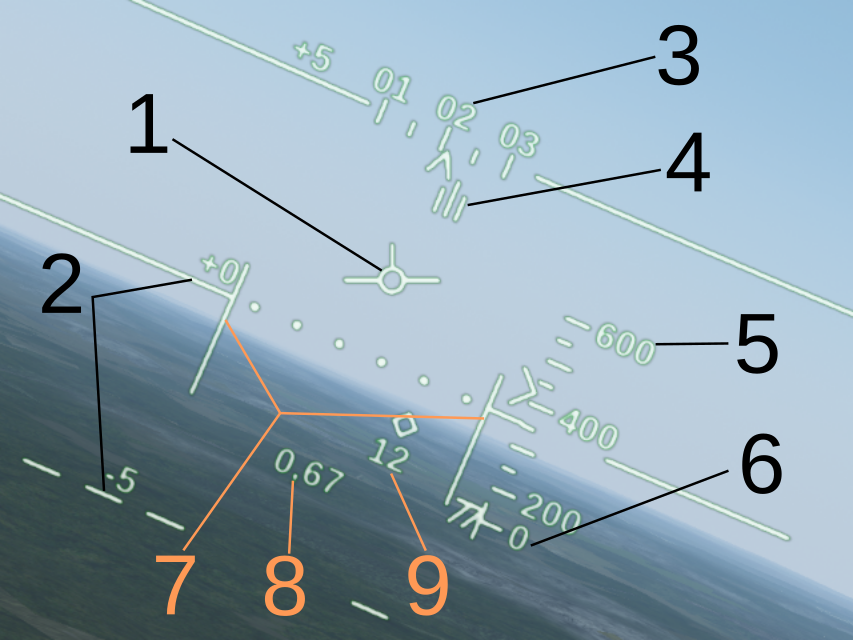
\includegraphics[width=0.7\textwidth]{images/displays/ja-hud-general.png}

  \begin{multicols}{2}
    \begin{enumerate}[nosep]
      \item \label{item:fpv} Flight path vector
      \item \label{item:horizon} Artificial horizon and pitch lines
      \item \label{item:heading} Heading scale
      \item \label{item:dest} Destination bearing
      \item \label{item:altitude} Altitude scale
      \item \label{item:rhm} Radar altimeter index and reference
      \item \label{item:altbars} Altitude bars
      \item \label{item:speed} Airspeed / Mach indicator
      \item \label{item:distance} Distance indicator
    \end{enumerate}
  \end{multicols}

  \caption{HUD overview}
  \label{fig:hud}
\end{figure}

\paragraph{Artificial Horizon (\cockpitref{fig:hud}{item:horizon})}
The artificial horizon and pitch scale provide an attitude reference.
The pitch scale consists of a line every 5 degrees.
Lines above the horizon are solid, lines below the horizon are dashed.
The artificial horizon itself is distinguished by six center dots.
Only the three pitch lines closest to the flight path vector are displayed.

\paragraph{Flight Path Vector (\cockpitref{fig:hud}{item:fpv})}
The FPV marker indicates the aircraft path direction relative to the ground.
Most of the HUD is centered around the FPV marker.

\paragraph{Heading Scale (\cockpitref{fig:hud}{item:heading})}
The heading scale is located above the FPV.
The fixed wedge index indicates aircraft track angle.
The second index consisting of 3 vertical lines
(\cockpitref{fig:hud}{item:dest}) indicates bearing to the next waypoint.

\paragraph{Altitude Scale (\cockpitref{fig:hud}{item:altitude})}
The altitude scale is located right of the FPV.
The fixed wedge index indicates aircraft altitude.
At low altitude the scale zooms in,
allowing to read the altitude more precisely for low level flight.

When the radar altimeter is active and in range,
the altitude 0 mark is displayed just below the altitude scale
(\cockpitref{fig:hud}{item:rhm}).
The radar altitude index, consisting of two wedges, can be read against this mark.
This can be used to set the altimeter QFE in flight.

\paragraph{Altitude Bars (\cockpitref{fig:hud}{item:altbars})}
The two altitude bars indicate the reference altitude
(also called commanded altitude) relative to the current altitude.

The top of the altitude bars represents commanded altitude,
while the artificial horizon represents current altitude.
If the top of the bars is on the horizon, the aircraft is at the commanded altitude.
If the top of the bars is above (resp.\ below) the horizon,
the aircraft is below (resp.\ above) the commanded altitude.

When the FPV is within 1\textdegree{} of the horizon,
the altitude scale index is fixed on the horizon.
Under these conditions, the top of the altitude bars
can be read on the altitude scale to obtain the commanded altitude.

Altitude bars are only displayed below 1000m.
When autopilot altitude hold is active, boxes are displayed together with
(below 1000m) or instead of (above 1000m) the altitude bars.

\subparagraph{Reference Altitude}
\label{sec:ref-alt}
The reference altitude displayed by the altitude bars is set as follows.
\begin{itemize}[noitemsep]
  \item During takeoff, the altitude bars are fixed over the horizon.
    After leaving takeoff mode, reference altitude is set to 500m.
  \item During flight, the reference button (keybinding \keys{\shift+R})
    sets the reference altitude to the current altitude.
  \item If autopilot altitude hold mode is active,
    the reference altitude is the autopilot altitude.
  \item When entering landing mode, reference altitude is set to 500m.
    It can still be modified with the reference button or by engaging autopilot altitude hold.
\end{itemize}

\paragraph{Airspeed / Mach Indicator (\cockpitref{fig:hud}{item:speed})}
Digital airspeed is displayed below the FPV,
with a minimum of 75km/h and a precision of 5km/h
(40kts and 1kts respectively in imperial units mode).
Above M 0.5, airspeed is replaced by a Mach indicator.

\paragraph{Distance Indicator (\cockpitref{fig:hud}{item:distance})}
Displays digital distance to the next waypoint.

\paragraph{Radar Altitude}
When radar altitude is less than 100m, it is displayed digitally
in the lower left part of the HUD, with the format e.g.\ `R 45'.
It is hidden for 30s after exiting takeoff mode, and in landing mode.

\paragraph{Ground Collision Warning}
Ground collision warning is displayed on the HUD as
a flashing arrow over the FPV, pointing in the pull-up direction.

\paragraph{Text Indications}
To the lower left of the FPV, plain text indications
can be shown in the following priority order:
\begin{enumerate}
  \item Altimeter setting warning `QFE' (flashing).
    At takeoff, indicates that the altimeter is incorrectly set.
    In flight, indicates that the altimeter should be switched to/from STD mode
    (assumes transition altitude 1500m).
  \item In landing mode, `TILS' indication when receiving ILS signal.
    (flashing if glideslope is not available or not in range).
  \item Selected weapon type (at the earliest 30s after leaving takeoff mode).
\end{enumerate}


\subsection{Takeoff Mode}
\begin{figure}[!ht]
  \centering
  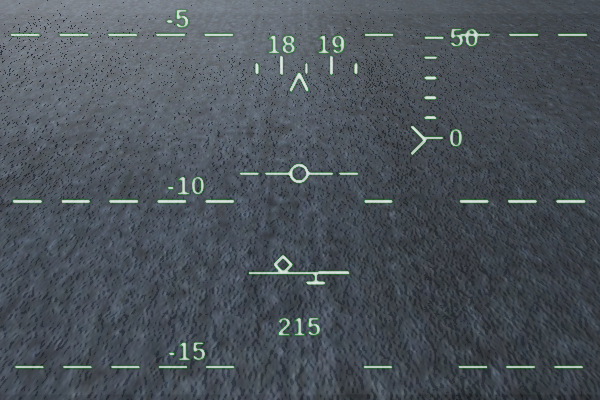
\includegraphics[width=0.5\textwidth]{images/displays/ja-hud-takeoff.png}
  \caption{HUD during takeoff}
  \label{fig:hud-takeoff}
\end{figure}

Takeoff mode is enabled when the nose gear is compressed.

During takeoff, the FPV is fixed vertically 10\textdegree{}
below the aircraft forward axis, and its symbol changes.
Horizontally, the FPV functions as in navigation mode,
and will e.g.\ move due to sidewind after rotation.

The distance line is displayed below the FPV, and represents airspeed.
The diamond upper index indicates aircraft speed,
and the inverted-T bottom marker indicates recommended rotation speed.
When the rotation angle reaches 5\textdegree{}, the distance line is hidden.

Takeoff mode stops once the airspeed exceeds M 0.35,
when the climb angle is at least 3\textdegree{},
or at landing gear retraction.

\subsection{Landing Mode}
\begin{figure}[!ht]
  \centering
  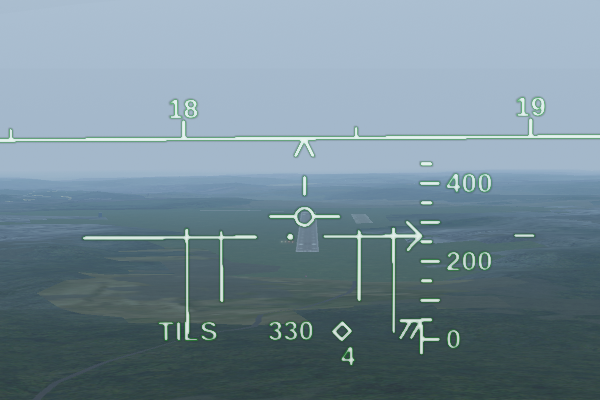
\includegraphics[width=0.5\textwidth]{images/displays/ja-hud-landing.png}
  \caption{HUD during final}
  \label{fig:hud-landing}
\end{figure}

In landing mode, the HUD changes when starting the final.
The -5\textdegree{} pitch line is removed,
and a glideslope line is added 2.86\textdegree{} below the horizon
(corresponding to a slope of 5\%).
Altitude scale, digital airspeed, and distance indicator are positioned around the glideslope line.
Heading scale is positioned over the horizon, and changes to a 1:1 scale.
Altitude bars are hidden.

If the climb or dive angle exceeds $\pm 7.5\degree$,
the default presentation of the pitch scale, digital airspeed, and distance indicator is restored,
while the heading and altitude scales are hidden.

\paragraph{Speed / AoA Indicator}
In landing mode, the vertical fin (`tail') of the flight path vector symbol
moves vertically to indicate deviation from the target speed or angle of attack.

The speed is correct when the bottom of the tail is on the FPV circle
(default position in navigation mode).
If the tail is higher than the circle, the aircraft speed is too high.
If the tail is lower (inside the circle), the aircraft speed is too low.

While the landing gear is up, the target speed is 550km/h.
Once the landing gear is down and locked, the target angle of attack is
computed based on aircraft weight, with a maximum of 12\textdegree{}
(15.5\textdegree{} if the button \cockpitref{fig:front-panel}{item:autothrottle-lights} is pressed and lit).

When the landing gear is down, the fin will blink if the angle of attack is critically high.

\paragraph{ILS Guidance}
If ILS guidance is used, the reference point on the glideslope line
indicates the heading to follow to align with the localizer.
Four vertical bars on the glideslope line indicate ILS glideslope deviation:
if the top of the bars is above, resp.\ below the glideslope line,
the aircraft is below, resp.\ above the ILS glideslope.

If ILS is not used (optical landing mode),
the reference point is aligned with the FPV, and the vertical bars are hidden.

\paragraph{Touchdown}
Below 35m, the HUD switches to optical landing display (ILS indications disappear).
Below 15m radar altitude, the HUD switches to flare mode.
The glideslope line moves up to indicate the descent angle
which gives a vertical speed of 2.8m/s, the maximum for touchdown.
If radar altitude is unavailable, transition to flare mode occurs at 35m.

Once the nose gear is compressed, the HUD switches to takeoff mode.

\subsection{Tactical Information}
Some tactical information is displayed on the HUD when a weapon is selected,
when a radar contact is tracked, and while in aiming mode.
%See \cref{chap:weapons} for details.
}


%\chapter{Systems}

% TODO: https://github.com/NikolaiVChr/flightgear-saab-ja-37-viggen/issues/120
%\section{Course Correction for Magnetic Deviation}
%Like in the real Viggen there are two ways to set the course correction, which makes sure that the instruments show true North instead of magnetic North (e.g. in north Norway the deviation is larger than 12\degree):
%\begin{itemize}
% \item Automatic: Simplified the computer averages the deviation between measured between 110 and 200 km/h during take-off.
% \item Manual: Make sure your airplane is properly aligned with the runway. Press FIXME. The reason for doing it manually is if the runway is slippery or there are strong crosswinds, which might change the way the nose points and therefore give a wrong deviation measurement. 
%\end{itemize}

%Please note that the computer in the real Viggen also makes some comparisons with the stored runway heading(s) to decrease the risk of failures. Warning light \emph{NAV SYST} would lit up. However, this is not modelled in FlightGear. 

%\AJSonly{Reference: [AJS\_1, sec. 20, ch. 3.4, p. 312]}

\part{Operation}
\chapter{Generic FlightGear Operations}
\section{Key Bindings}
A summary of the key bindings can also be found in \menu{Help>Aircraft Help}.

\paragraph{General}
\begin{description}
\AJSonly{
  \item[\keys{M} / \keys{\shift+M}] Rotate main mode selector knob clockwise/counterclockwise.
  \item[\keys{K} / \keys{J}] Extend/retract airbrakes (press for ca.\ 2s for full extension).
    When the landing gear is down, airbrakes retract as soon as \keys{K} is released.
  \item[\keys{\ctrl+B}] Toggle airbrakes (simplified airbrakes control).
    When the landing gear is down, airbrakes retract as soon as \keys{\ctrl+B} is released.
}
  \item[\keys{\backspace}] Toggle thrust reverser.
  \item[\keys{\shift+PageUp} / \keys{\shift+PageDown}] Raise/lower seat position.
  \item[\keys{\ctrl+O}] Open/close canopy.
  \item[\keys{\ctrl+E} $\times3$] Eject
  \item[\keys{J}] Jettison drop tank (in flight only).
  \item[\keys{\shift+S}] Acrobatic smoke.
  \item[\keys{\ctrl+Y}] Display landing airport informations (requires runway selected in route manager).
\end{description}

\paragraph{Displays}
\begin{description}
  \item[\keys{\shift+R}] Set reference altitude (cf.~\cref{sec:ref-alt}) \JAonly{/ toggle IR missile boresight mode}.
\ifbool{AJS}{
  \item[\keys{H}] Toggle HUD up/down position.
  \item[\keys{I}] Toggle HUD low altitude declutter (cf.~\cref{sec:hud-slav-switch}).
  \item[\keys{\shift+I}] Toggle radar or barometric altitude on HUD and CI (cf.~\cref{sec:hud-slav-switch}).
}{
  \item[\keys{H}] Toggle HUD aiming mode / engage visual landing mode.
  \item[\keys{\shift+I}] Toggle between english/imperial and swedish/metrics display modes.
  \item[\keys{\shift+Y}] Engage landing mode.
}
  \item[\keys{\shift+H}] Cycle HUD brightness.
  \item[\keys{Y}] Use flight controls to controls cursor.
\JAonly{
  \item[\keys{L}] Cursor click.
  \item[\keys{\shift+M}] Switch cursor between MI and TI.
}
\end{description}

\paragraph{View}
\begin{description}
  \item[\keys{\shift+Q}] Reset view.
  \item[\keys{\ctrl+Q}] Zoom on radar display.
  \item[\keys{\ctrl+\shift+Q}] Zoom on HUD.
\end{description}

\paragraph{Autopilot}
\begin{description}
  \item[\keys{\ctrl+T}] Autopilot stability assist mode.
  \item[\keys{\ctrl+W}] Autopilot attitude hold mode.
  \item[\keys{\ctrl+A}] Autopilot altitude hold mode.
  \item[\keys{\ctrl+D}] Disengage all autopilot modes.
  \item[\keys{\ctrl+S}] Toggle autothrottle lever.
  \item[\keys{U}] Autothrottle quick disengage \AJSonly{(gear up: IR missile quick select)}.
  \item[\keys{\ctrl+\arrowkeyleft} / \keys{\ctrl+\arrowkeyright}] Trim yaw, or adjust autopilot heading/bank angle.
\end{description}

\paragraph{Radar Controls}
See also \cref{sec:cursor}.
\begin{description}
\ifbool{AJS}{
  \item[\keys{R} / \keys{F}] Radar on/off.
}{
  \item[\keys{R}] Toggle radar. In aiming mode: turn radar off.
}
  \item[\keys{[} / \keys{]}] Decrease/increase radar range (positions: 15km, 30km, 60km, 120km).
  \item[\keys{<} / \keys{>}] Adjust radar elevation down / up.
\ifbool{AJS}{
  \item[\keys{\shift+F}] Memory mode.
  \item[\keys{\ctrl+F}] Terrain navigation mode.
  \item[\keys{\{} / \keys{\}}] Decrease/increase radar picture gain.
}{
  \item[\keys{\shift+F}] Wide scan mode.
  \item[\keys{\ctrl+F}] TWS (Track While Scan) mode.
  \item[\keys{F}] Toggle STT (Single Target Track) or TWS mode.
    When a primary target is selected, this directly toggles between the two modes.
    If the MI cursor is active, it instead changes the radar mode which will be obtained after designating a contact.
  \item[\keys{\shift+N}] Engage aiming mode, radar disk search mode with auto-lock (`dogfight mode').
  \item[\keys{M}] Cycle TWS primary target.
  \item[\keys{N}] IFF interrogation.
}
\end{description}

\AJSonly{
\paragraph{Radar Stick}
\begin{description}
  \item[\keys{O}] Press T1 (radar stick click stage 1).
  \item[\keys{\shift+O}] Toggle T1 \textit{holding}.
  \item[\keys{L}] TV select/click.
\end{description}
}


\paragraph{Combat}
\begin{description}
\ifbool{AJS}{
  \item[\keys{C} / \keys{\shift+C}] Rotate weapon selector knob clockwise/counterclockwise.
  \item[\keys{U}] IR missile quick select (gear down: autothrottle quick disengage).
}{
  \item[\keys{C}] Missile quick select.
  \item[\keys{\shift+C}] Cannon quick select.
}
  \item[\keys{\shift+E}] Toggle trigger safety.
  \item[\keys{E}] Fire weapon.
  \item[\keys{\shift+U}] Uncage IR missile seeker (requires lock). Hold for ~1s: cage/reset IR missile seeker.
\ifbool{AJS}{
  \item[\keys{(} / \keys{)}] Decrease/increase A/A sight wingspan / bomb interval.
}{
  \item[\keys{(} / \keys{)}] Decrease/increase cannon sight wingspan.
  \item[\keys{\{} / \keys{\}}] Decrease/increase cannon sight distance.
}
  \item[\keys{Q}] Release flare/chaff.
\end{description}

\subsection{Radar Stick Controls}
\label{sec:cursor}
The radar stick is used to control the cursor on the \ifbool{AJS}{CI}{MI and TI}.
There are three ways to control it:
\begin{itemize}
  \item Enable the option \menu{\ifbool{AJS}{AJS-37}{JA-37Di}>Options>Arrow keys control radar cursor},
    and use the arrow keys to move the cursor, \keys{\return} to click/select.
  \item Add joystick bindings to control the cursor.
    This can be done under \menu{File>Joystick Configuration},
    the controls are named \menu{Cursor Horizontal}, \menu{Cursor Vertical}, and \menu{Cursor Click}.
    Alternatively, manually edit joystick configuration files to bind the properties
    \begin{alltt}
/controls/displays/cursor-slew-x
/controls/displays/cursor-slew-y
/controls/displays/cursor-click\end{alltt}
  \item Press \keys{Y} to use the main flight controls
    (joystick, mouse, arrow keys, whatever you use to control the aircraft)
    to instead control the cursor.
    In this mode, elevator and aileron controls are used to move the cursor.
    Normal flight controls are restored by pressing \keys{Y} again.
    A ground collision warning will also immediately restore normal flight controls.

    Consider using autopilot when controlling the cursor in this way.
\end{itemize}

In all cases, \keys{L} can also be used to click.

\AJSonly{%
  The same controls are used to move and lock the Rb 75 seeker,
  and to fly the Rb 05A remote controlled missile.
}

\section{\variant{} Menu}
The menu \menu{\ifbool{AJS}{AJS-37}{JA-37Di}} contains Viggen-specific dialogs and menus.
The following entries are present.
\begin{description}
  \item[\menu{Manual (open in browser)}] Open this manual in a browser or PDF reader.
  \item[\menu{Select Livery}] There is a variety of liveries available, both historical and fictional.
  \item[\menu{Auto start/stop}] Lets you start and stop the plane without needing to switch switches etc.\ yourself.
    The progress is shown in the top centre of the screen in blue text.
    The final notification of the start-up sequence is `Engine ready'.
    The shut-down sequence is done, when the aircraft is dark.
  \item[\menu{Repair}] Repairs system failures.
    In case of a full crash, this option is of limited use;
    one should restart instead with \menu{File>Reset}.
\AJSonly{\item[\menu{Ground Crew Panel}] Ground crew weapon panel.}
  \item[\menu{Performance monitor}] Display aircraft performance (mostly for development).
  \item[\menu{Systems monitor}] Display internal status of some systems (mostly for development).
  \item[\menu{Combat log}] Multiplayer damage log (damage dealt and received).
  \item[\menu{Load radio channels}] Load configuration files for programmable radio channels.
\JAonly{\item[\menu{Friends (IFF)}] Allows to set a list of friendly callsigns for IFF (cf.\ \cref{sec:iff}).}
  \item[\menu{Toggle chocks}] Parking chocks. Only available when fully stopped.
  \item[\menu{Toggle external power}] External electrical power, normally used for startup.
    An electrical power truck is shown to the right of the aircraft when enabled.
    Only available when fully stopped.
  \item[\menu{Options}] Viggen specific configuration options, see \cref{sec:options-dialog}.
\end{description}


\section{\variant{} Options}
\label{sec:options-dialog}
The dialog \menu{\ifbool{AJS}{AJS-37}{JA-37Di}>Options} contains the following configuration options.
\begin{description}
  \item[\menu{Head shaking}] Head shaking during ground roll and at high alpha.
    May conflict with other view control scripts, e.g.\ headtracking.
  \item[\menu{Cockpit labels in Swedish}] Enable historical Swedish cockpit,
    instead of the English translation.
    (Cockpit translation is incomplete.)
\JAonly{

    This option is for \emph{physical labels} only, and should not be confused
    with the next one which affects displays.
  \item[\menu{HUD/TI in metric units and Swedish}]
    Change the unit system and language used in displays.  Shortcut: \keys{\shift+I}.

    This option is for \emph{displays} only, and should not be confused with
    the previous one which affects physical labels.
  \item[\menu{TI: show non-functional menu items}]
    On the TI (HSD), show non-implemented menus.
  \item[\menu{TI Display: use Internet to fetch map}]
    Enable download of the world map displayed on the TI (HSD).
}
\AJSonly{
  \item[\menu{Ground radar quality}]
    Adjusts the resolution of the AJS ground radar. This significantly affects performances.
  \item[\menu{Automatic ground crew weapon panel settings}]
    Automatically adjust ground crew weapon panel for current loadout.
}
  \item[\menu{Arrow keys control radar cursor}]
    When enabled, the arrow keys will control the radar stick to move the
    cursor on the different displays, and \keys{\return} is used to `click'
    (select the target under the cursor, or other depending on context).

    When disabled, the arrow keys are used for elevator and aileron,
    and \keys{\return} is used for rudder (FlightGear default behaviour).
    Cf.\ \cref{sec:cursor} for more details regarding cursor controls.
  \item[\menu{Enable multiplayer damage}]
    Allows to deal and receive damage from other compatible aircrafts
    (other Viggens, F-14, F-15, F-16, M-2000, MiG-21, etc.) in multiplayer.
    This requires \emph{both} involved aircraft to enable damage.

    For fairness, this option can only be toggled when stopped on the ground.
    It also enforces some realism options: blackout, normal simulation speed,
    no external views, and disabling fuel, payload, repair, and combat log menus while in flight.
\end{description}


\chapter{Standard Procedures}
To come! Please check FlightGear built-in checklists
\menu{Help>Aircraft Checklists} in the meantime.

%\chapter{Emergency Procedures}

\chapter{Weapons Operation}
\label{chap:weapons}
\AJSonly{
\section{Loadout Restrictions}
\label{sec:loadout}
While the AJS 37 has access to a wide variety of weapons, they can not all be loaded at the same time.
The following restrictions apply:
\begin{enumerate}
  \item \label{rule:unique} Only one type of primary weapon can be loaded at any time.
  \item Primary weapons are everything except IR missiles (Rb 24, Rb 24J, and Rb 74 Sidewinders).
    Any combination of IR missiles can be loaded in addition to the primary weapons.
  \item There is an exception to rule~\ref{rule:unique}:
    AKAN gun pods can be loaded together with either Rb 05 or Rb 75 missiles
    (but not Rb 05 and Rb 75 together).
\end{enumerate}

Loading weapons which violate these restrictions triggers a warning text message,
and will result in \emph{all} weapons being unusable.

In the \menu{Equipment > Fuel and Payload} dialog,
the \menu{Loadout Presets} allows to quickly load several combinations of weapons,
and gives a good overview of the allowed loadouts.
}

\section{General Procedures}
The generic weapon employment procedure is the following.
\begin{enumerate}
  \item Select weapon type with%
    \ifbool{AJS}{
      the weapon selector knob (\keys{C} / \keys{\shift+C}), cf.\ \cref{sec:weapon-panel}.
      Alternatively, press \keys{U} for A/A missiles quick selection.
    }{
      \keys{C} (A/A missiles), \keys{\shift+C} (cannon), or through the TI.
    }
  \ifbool{AJS}{
  \item Set main mode selector to ANF/CBT
    (\figref{fig:left-panel}{item:main-mode}, \keys{M} / \keys{\shift+M}).
  }{
  \item If desired, engage aiming mode with \keys{H}.
  }
  \item \ifbool{AJS}{Depending on the weapon type,}{For missiles,} lock on to the target.
  \item Open trigger safety with \keys{\shift+E} to arm the selected weapon.
  \item Fire the weapon with \keys{E}. \JAonly{Press and hold for ca.~1 second to fire missiles.}
  \item Secure the trigger with \keys{\shift+E}.
\end{enumerate}

Remarks:
\begin{itemize}
  \item Upon switching to \ifbool{AJS}{mode ANF/CBT}{aiming mode},
    the HUD changes to a weapon-specific aiming presentation.
    \AJSonly{For the Rb 04, Rb 15, Rb 05, and m/90,
    this aiming mode is the same as the usual navigation HUD.}
  \item It is possible to fire \ifbool{AJS}{in mode NAV instead of ANF/CBT}{without using the aiming mode}.
    In this case, \ifbool{AJS}{the aiming presentation}{a simplified aiming presentation}
    is engaged when opening the trigger safety.
\end{itemize}

\subsection{Trigger Safety Usage}
The trigger safety role is not just to prevent unintentional fire.
It is an important part of the fire control system as it arms the weapon.
Improper use of trigger safety will prevent weapon usage.

General guidelines are:
\begin{itemize}
  \item Only open the trigger safety once the target is in sight / on radar,
    and the decision to engage it has been made.
  \item Only open the trigger safety after the desired weapon is selected.
    If a new weapon is selected while the trigger is unsafe, the new weapon
    will not be armed (until the trigger is secured and unsecured again).
  \item Secure the trigger shortly after firing.
  \item When firing several missiles in succession, the trigger must be secured between each weapon.
\end{itemize}

\ifbool{AJS}{\section{AKAN and ARAK}
The m/55 AKAN cannon pods and m/70 ARAK rocket pods share
the same sighting mechanisms and firing procedures.

The m/55 AKAN is a 30mm ADEN cannon pod, with 150 rounds.
Two can be carried on the main wing pylons.

The m/70 ARAK consists of six 135mm rockets, which are all fired in a 0.6 seconds salvo.
Four pods can be carried on the main wing and fuselage pylons.

\subsection{Ranging}
The AJS combines two methods to compute the distance to the target
(i.e.\ the point on which the aiming reticle is located).

\paragraph{Ranging by Triangulation}
Triangulation computes the distance to the target based on aircraft altitude
and the angle between the aiming reticle and the horizon.
Ranging by triangulation assumes that the target altitude is 0,
thus it is essential to properly calibrate indicated altitude by
1.\ setting the altimeter to the target QFE,
or 2.\ using radar-altimeter corrected altitude (switch HÖJD CI SI in position RHM).

Ranging by triangulation is only available if the aiming reticle is at
least 5\textdegree{} below the horizon.

\paragraph{Radar Ranging}
The aircraft main radar is used to compute the range to the ground.
Radar ranging is only used when the following conditions are met.
\begin{itemize}[nosep]
  \item Triangulation ranging is active, and computed distance is at most 7km.
  \item Main mode selector is ANF/CBT.
  \item Roll angle is less than 45\textdegree{}, or trigger safety is open.
\end{itemize}

\paragraph{Remarks}
Because triangulation ranging is required before radar ranging can be enabled,
it is essential to at least approximately calibrate the altimeter.

If triangulation ranging is unavailable (reticle is less than 5\textdegree{} below the horizon)
a fixed distance of 1400m is used to compute reticle position.

\subsection{HUD Aiming Mode}
\begin{figure}[!ht]
  \centering
  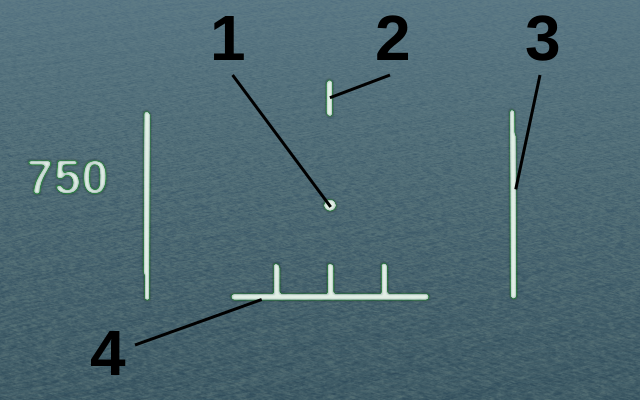
\includegraphics[width=0.45\textwidth]{images/displays/ajs-hud-aiming1.png}
  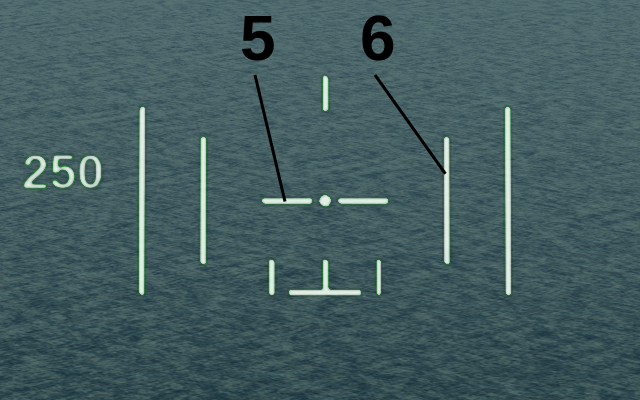
\includegraphics[width=0.45\textwidth]{images/displays/ajs-hud-aiming2.png}

  \begin{multicols}{2}
    \begin{enumerate}[nosep]
      \item \label{item:reticle} Aiming reticle
      \item \label{item:rdr-range} Radar ranging mark.
      \item Side bars, no functionality.
      \item \label{item:distline} Distance line.
      \item \label{item:fire-mark} Firing command lines.
      \item \label{item:pullup-bars} Evasion warning bars.
    \end{enumerate}
  \end{multicols}
  \caption{HUD aiming mode}
  \label{fig:hud-aiming}
\end{figure}

When AKAN or ARAK are selected, the HUD aiming mode (\cref{fig:hud-aiming})
is enabled by switching to mode ANF/CBT, or arming the weapon (trigger unsafe) in mode NAV.

It comports an aiming reticle (\figref{fig:hud-aiming}{item:reticle}),
the digital altitude indicator, and a number of indicators and cues for target range,
which appear in the following order:
\begin{enumerate}
  \item The distance line (\figref{fig:hud-aiming}{item:distline})
    indicates range to the target up to 8km when triangulation ranging is active.
    The side marks indicate the computed firing distance
    (minimum firing distance giving sufficient time for safe evasion).
  \item When radar ranging is active, a vertical bar is displayed above the reticle
    (\figref{fig:hud-aiming}{item:rdr-range}).
  \item 2 seconds before computed firing distance, the distance line blinks.
  \item 0.5 seconds before computed firing distance, the firing command lines appear
    (\figref{fig:hud-aiming}{item:fire-mark}).
  \item When the minimum distance for safe evasion is passed,
    the evasion warning bars start blinking (\figref{fig:hud-aiming}{item:pullup-bars}).
    This indicates that the attack run should be aborted immediately.
\end{enumerate}

Minimum distance for safe evasion is computed to keep the aircraft out of the
explosion debris zone, and assumes a 5g pull, with some margin.

The position of the aiming reticle is correct starting 3 seconds before computed firing distance.
The aiming reticle includes wind compensation.


\section{Rb 75}
The Rb 75 is a Swedish version of the AGM-65A television-guided missile.
It is designed for use against ground targets.
The pilot locks on the target by manually slewing the Rb 75 seeker head using the radar stick.

In the real Viggen, the EP-13 screen to the right of the HUD displayed the Rb
75 seeker image, and was used to lock on the target.

In FlightGear, the EP-13 screen is not functional.
Instead, the seeker position is displayed as a small circle on the HUD.
The seeker is controlled with the radar stick (see \cref{sec:cursor}).
When the seeker is over the target, it can be locked using the radar stick click/select.

\section{Rb 05A}
The Rb 05A is a remote-controlled missile.
It is primarily intended for use against ground and naval targets,
but can also be used against slow-manoeuvring air targets thanks to a proximity fuse.
The missile is guided visually by the pilot.
A flare at the back of the missile helps the pilot to keep sight of it (\cref{fig:rb05-flare}).

\begin{figure}
  \centering
  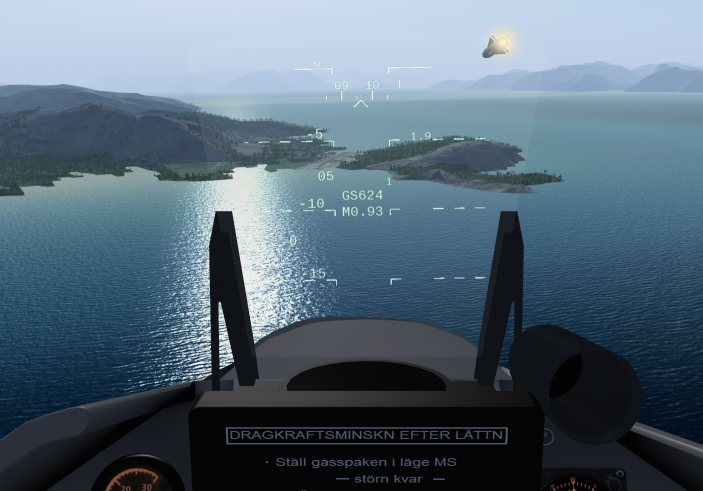
\includegraphics[height=0.3\textwidth]{images/weapons/rb_05a_start_popup.png}
  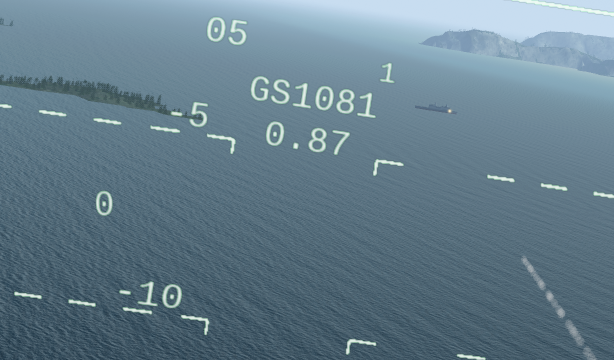
\includegraphics[height=0.3\textwidth]{images/weapons/rb_05a_before_impact_ship.png}
  \caption[Rb 05A flare for visual guidance]{Rb 05A flare for visual guidance.
    On the left, the missile is entering the pilot's field of view just after launch.
    On the right, the missile is about to hit the target ship,
    and the missile flare is visible over the ship
  }
  \label{fig:rb05-flare}
\end{figure}

In FlightGear, the Rb 05A uses the same controls as the radar stick, cf.\ \cref{sec:cursor}.\footnote{%
  In the real Viggen, a separate control stick on the right console was used.
}

\subsection{Procedure}
\begin{enumerate}
  \item Main mode selector to ANF/CBT.
    (\figref{fig:left-panel}{item:main-mode}, shortcuts \keys{M}/\keys{\shift+M}).
  \item Select the Rb 05A (cycle weapons with \keys{C}).
  \item Once in firing position, consider engaging autopilot in ATT or HÖJD/ALT mode to reduce pilot workload.
  \item Identify the target visually.
  \item Unsafe the trigger and fire within 9km of the target.
  \item After 1.7s, missile controls are enabled
    (cf.\ \cref{sec:cursor} for control methods).
    At this point, it should be well within the pilot field of view.
  \item When the missile hits, take evasive manoeuvres, secure the trigger, and switch to NAV mode.
\end{enumerate}

Remarks.
\begin{itemize}
  \item Recommended speed is 700-1150 km/h.
  \item Recommended attitude is a level flight or slight dive,
    so as to not loose sight of the target and the missile.
  \item Recommended altitude is 300-400 meters above ground.
  \item The target do not need to be directly in front of the aircraft
    as the missile can be guided considerably to the side.
    However, doing so makes it harder to aim the missile, and reduces effective range.
  \item The missile flies for ca.\ 24 seconds, giving it a maximum effective range of ca.\ 9 km.
  \item It is easiest to aim the missile using the collimation principle:
    try to keep the missile flare covering the target at all time.
\end{itemize}
}{}

\appendix
\chapter{Viggen Swedish Dictionary}
\begin{tabular}{ll@{\hspace{1em}}l}
  & Swedish & English \\
  \hline
  & TILL & ON \\
  & FRÅN & OFF \\
  Instruments:\\
  & Höjd & Altitude \\
  & Fart & Speed \\
  & Kurs & Course/Heading \\
  & Varv & Revolution (RPM) \\
  & Bränsle & Fuel \\
  Autopilot: \\
  & SPAK & Stability assist mode (lit.\ Stick) \\
  & ATT & Attitude hold \\
  & HÖJD & Altitude hold \\
  & AFK (Automatisk FartKontroll) & Auto-throttle \\
  Displays: \\
  & SI (SiktlinjesIndicator) & HUD \\
  & CI (CentralIndicator) & AJS radar screen \\
  & MI (MålIndicator) & JA radar screen (lit.\ Target Display) \\
  & TI (TaktiskIndicator) & JA Horizontal Situation Display \\
\end{tabular}
\end{document}

%\url{https://www.aef.se/Flygvapnet/Tidskrifter/FV_Nytt/Flygvapennytt_1993-2.pdf} has an article and 2 pictures about the automatic aiming mode for the cannon in the JA version (in Swedish).


\chapter{References}

A comprehensive book in English covering all variants is \glqq Saab 37 Viggen --- The ultimate portfolio\grqq by Jan Jørgensen (published in 2014 by \href{http://www.nordicairpower.com/}{Nordic Airpower}).

\subsection{Original Manuals}
A significant part of the original manuals are available on the internet, and in recent years also many of the formerly classified chapters (as far as the information is not still valid due to (re-)use in the Gripen) have been become available. As the Viggen could not be sold to other countries\footnote{Austrian pilots went through a training programme on the Viggen to familiarise with modern combat airplane, but never bought it}, a significant part of the text and illustrations are in Swedish.

The following manuals are core to the understanding of flying a Viggen in military operations. Where possible, references are made in this manual to text elements in the original manuals(e.g. [AJS\_Del1, sec. 20, ch. 3.4.2, p. 312]). Also, this manual does typically not repeat illustrations from the original handbooks, but shows a screenshot from the simulation instead, so you can compare.

\begin{table}[!th]
\begin{tabular}{|l|l|c|r|}
\hline
Ref & Title & Date & Pages \\
\hline
AJ\_Del2 & FPL AJ37 Speciell Förarinstruktion Del 2 kap 1 (M5800--370011) & 1975--02--01 & 181 \\
AJS\_Del1 & FPL AJS37 Speciell Förarinstruktion Del 1 (M5800--370011) & 1994--11--15 & 517 \\
AJS\_Del2 & FPL AJS37 Speciell Förarinstruktion Del 2 (M5800--370011) & 1994--11--01 & 222 \\
AJS\_Del3 & FPL AJS37 Speciell Förarinstruktion Del 3 (M5800--370011) & 1994--11--15 & 295 \\
JA\_Vol1 & Flight Manual A/C JA37 Volume 1 (M5800-370051) & 1999--01--20 & 497 \\
\hline
\end{tabular}
\caption{Overview of flight manuals from the original Viggen}
\end{table}

\subsection{FlightGear Related}
\begin{itemize}
\item The \href{http://wiki.flightgear.org/Saab_37_Viggen}{FG wiki article} contains a comprehensive feature overview, links to forum articles etc. However, the wiki is not always up to date.
\item \href{http://opredflag.com/}{Operation Red Flag (OPRF)} is a FlightGear military simulation community discussing, developing and using many of the combat features in the Viggen.
\item On Discord there is a dedicated \href{https://discord.gg/jc5pSM5}{Viggen server} and a \href{https://discord.gg/SmGFnJN}{OPRF server}. Say hello and discuss the Viggen's features, development and your flight experience. Preliminary help with issues can be gotten as well, confirmed issues should be reported in the Viggen's \href{https://github.com/NikolaiVChr/flightgear-saab-ja-37-viggen/issues}{issue tracker} for resolution.
\item The \href{https://www.youtube.com/playlist?list=PLogi97V-ki0GfCLqimTtIq9RIVcm-GRFE}{Flightgear Saab 37 Viggen YouTube Playlist} includes amongst others a set of tutorial videos featuring the JA and the AJS variant.
\end{itemize}

\subsection{Other Combat Flight Simulators}
Both \href{https://www.digitalcombatsimulator.com/en/index.php}{DCS} and \href{https://www.benchmarksims.org/}{BMS Falcon} have flyable Viggens. Especially for DCS there is an abundance of resources available on the internet (e.g. YouTube). Please note that while there can be valuable additional information and context provided in content from other simulators, the capabilities modelled will differ.

\subsection{Swedish Documentation Sites}
\begin{itemize}
\item Arboga Elektronikhistoriska Förening: \url{https://www.aef.se}, e.g. 
\begin{itemize}
\item \href{https://www.aef.se/Avionik/Notiser/PS-37/PS-37A.htm}{Spanings- och siktesradar PS-37/A (for the AJS)}
\item \href{https://www.aef.se/Avionik/Notiser/Siktesradar_PS-46_1.htm}{Flygradarinstallation JA37 ---Siktesradar PS46} (includes links to 2 articles from Ericsson)
\item \href{https://www.aef.se/Flygvapnet/Tidskrifter/FV_Nytt/FVN_oversikt.htm}{FlygvapenNytt 1960 – 2003}: \url{https://www.aef.se/Flygvapnet/Tidskrifter/FV_Nytt/Flygvapennytt_1991-2.pdf} announced the AJS Viggen and \url{https://www.aef.se/Flygvapnet/Tidskrifter/FV_Nytt/Flygvapennytt_1994-4.pdf} had follow-up articles.
\end{itemize}
\item Digitalt Museum: \url{https://digitaltmuseum.se/}:
\begin{itemize}
\item Aeroseum Göteborg: \url{https://digitaltmuseum.se/owners/S-AER}
\item Flygvapenmuseum: \url{https://digitaltmuseum.se/owners/S-FV}
\item Teknikland: \url{https://digitaltmuseum.se/owners/S-TL}
\item Sveriges militärhistoriska arv: \url{https://digitaltmuseum.se/owners/S-MHA}
\end{itemize}
\end{itemize} 


\begin{landscape}
\chapter{Viggen Related Videos}
The following selection of videos has been made based on operational content or visibility of details. There exist many more videos --- some of which with higher quality from recent air shows. If you miss a video below, let us know.

\begin{table}[!th]
\begin{tabular}{|p{5cm}|c|c|c|p{9cm}|}
\hline
Title & Length & Subtitles & Year & Comments \\
\hline

\href{https://www.youtube.com/watch?v=kBq5qA8r4dA}{SF/SH37 \& JA37 VIGGEN at F13 Wing} & 18 min & yes & 2000 & Mostly about the reconnaissance and photo version\\
\href{https://www.youtube.com/watch?v=0sRACNVVmpE}{Saab 37 Viggen 2001 1-2} & 15 min & no & ?? & Historic part plus early versions\\
\href{https://www.youtube.com/watch?v=pAPteuBsRGg}{Saab 37 Viggen 2001 1-2} & 14 min & no & ?? & Mostly about the evolution of the JA. Some footage of HUD and CI/TI screens.\\
\href{https://www.youtube.com/watch?v=fmqXa0oetUA}{VI FLÖG HÅRT OCH STRIDSMÄSSIGT} & 15 min & no & ?? & A fighter pilot tells stories\\
\href{https://www.youtube.com/watch?v=ErK3zaNRccE&}{Jaktviggenpilot på Bråvallajakten} & 14 min & no & 1989 & A day in the live of a fighter pilot\\
\href{https://www.youtube.com/watch?v=qaNt9_sQdGI}{Kurvstrid (Dogfight) SAAB JA37C VIGGEN} & 8 min & yes & ?? & Various dogfights with some HUD visibility\\
\href{https://www.youtube.com/watch?v=oB6-jJEWjWk}{S som i Speed - Göran flyger Viggen} & 6 min & no & 1996 & Some low level flying\\
\href{https://www.youtube.com/watch?v=gwgJNdWZlj0}{SH-37 Viggen Sea Surveillance} & 4 min & n/a & ?? & Some nice sequences of the AJS CI and a few glipse of the HUD\\
\href{https://www.youtube.com/watch?v=mgPS5-SbI0c}{Viggen attackuppdrag} & 2 min & no & ?? & Attack with rockets using pop-up method. Some sequences of the HUD.\\
\href{https://www.youtube.com/watch?v=eQjAp7bTnUg}{Kalla Krigets Fordon avsnitt 6: SAAB 37 Viggen} & 9 min & no & 2016 & A bit of history and relation between the plane and the road base system. During the very last seconds some close-up sequences of the CI.\\
\href{https://www.youtube.com/watch?v=slm9ksxU0HY}{Viggen Road base exercise} & 6 min & n/a & ?? & As the title says.\\
\href{https://www.youtube.com/watch?v=hWrsP3hq5M8}{AJ-37 Viggen Low Level Flying} & 4 min & n/a & ?? & As the title says. Some HUD sequences incl. rocket attack.\\
\href{https://www.youtube.com/watch?v=UOszNlNeRVs}{SAAB 37 Viggen} & 4 min & n/a & ?? & Some nice air ballet plus a few sequences of the CI.\\
\href{https://www.youtube.com/watch?v=IbsYsUvCy7s}{Rörlig klargöring JA37 Arlanda} & 43 min & no & 1996 & Ground operations of JA 37 on an improvised stand at Arlanda airport\\
\href{https://vimeo.com/60091080}{Viggen i Älskar, älskar inte} & 4 min & no & ?? & Excerpts from the feature film, Älskar, älskar inte. Nice dogfighting between JA and AJS plus some CI sequences\\
\href{https://www.youtube.com/watch?v=eT00_OVrv7o}{JA-37 and SK-37E Night Ops} & 7 min & no & ?? & Night flying with good pictures of exhaust, navigation and beacon lights\\
\href{https://www.youtube.com/watch?v=0ocSUd9_5Tw}{JA37 F21 1982-2004} & 17 min & no & ?? & Around min 5 and 15 there are longer sequences of the HUD in weapons mode (JA variant)\\

\hline
\end{tabular}
\caption{Selected videos featuring the Viggen. Unless described otherwise in the comments, the language is Swedish}
\end{table}

% Videos watched but not found interesting enough
% \href{https://www.youtube.com/watch?v=rFZKvO95bQ0}{2018-10-17 Svensk stridspilot under det kalla kriget}
% \href{https://www.youtube.com/watch?v=RHVzkVwI68w}{Vetenskapens Värld - Viggen} Mostly project and politics history until first viggen operational
% \href{https://www.youtube.com/watch?v=M8HF1gH0MPc}{37 Viggen - The Power of Viggen!} Mostly flight display
% \href{https://www.youtube.com/watch?v=Z_EnkvE6LZA}{Fredens Hav}
\end{landscape}

